\documentclass[a4paper,12pt]{report}
\usepackage[utf8x]{inputenc}

\usepackage{amsmath}
\usepackage{amssymb}
\usepackage{graphicx}
\usepackage{subcaption}
\usepackage{verbatim}
\usepackage{mathtools}
\usepackage{subcaption}
\usepackage[titlenumbered,ruled,linesnumbered]{algorithm2e}
\usepackage{todonotes}
\usepackage{booktabs}

\usepackage[UKenglish]{babel}

\usepackage{hyperref}
\hypersetup{
    citecolor=black,
    filecolor=black,
    linkcolor=green,
    urlcolor=black
}
\usepackage{subcaption}
\usepackage{flexisym}
\usepackage{listings}
\usepackage{color}

\definecolor{dkgreen}{rgb}{0,0.6,0}
\definecolor{gray}{rgb}{0.5,0.5,0.5}
\definecolor{mauve}{rgb}{0.58,0,0.82}

\lstset{frame=tb,
  language=Python,
  aboveskip=3mm,
  belowskip=3mm,
  showstringspaces=false,
  columns=flexible,
  basicstyle={\small\ttfamily},
  numbers=none,
  numberstyle=\tiny\color{gray},
  keywordstyle=\color{blue},
  commentstyle=\color{dkgreen},
  stringstyle=\color{mauve},
  breaklines=true,
  breakatwhitespace=true,
  tabsize=3
}

\pagenumbering{roman}

\begin{document}

%-------------------------------------------------------------------------------
% Title Page
%-------------------------------------------------------------------------------
\begin{titlepage}
\center % Center everything on the page

% Logo section
\vspace{-1cm}

\includegraphics[width=4cm]{img/logoUHi.jpg}
\vspace{2cm}

% Title section
{ \Large \bfseries Title of The Thesis: First Line}\\  % Title of your document
\vspace{0.5cm}
{ \Large \bfseries Title of The Thesis: Second line}\\ % Title of your document
\vspace{0.5cm}
\vspace{2cm}

% Author section
\begin{minipage}{0.49\textwidth}
\begin{flushleft} \large
\emph{Author:}\\
FirstName \textsc{LastName} \\ % Name of the student
StudentID \\ % Your maticulation number
\end{flushleft}
\end{minipage}
~
\begin{minipage}{0.46\textwidth}
\begin{flushright} \large
\emph{Supervisors:} \\
FirstName \textsc{LastName} \\ % 1st Supervisor's Name
FirstName \textsc{LastName} % 2nd Supervisor's Name
\end{flushright}
\end{minipage}\\
\vspace{2cm}

% Date section
{ \today}\\ % Date, change the \today to a set date if you want to be precise
\vspace{1cm}

% University Section
{ \large \bfseries Thesis submited for}\\  % Title of your document
\vspace{0.3cm}
\textsc{\Large Master of Science in Data Analytics}\\% Major heading such as course name
\vspace{1cm}
\textsc{\large Wirtschaftsinformatik und Maschinelles Lernen}\\ % Name of your university/college
\vspace{0.3cm}
\textsc{\large Stiftung Universität Hildesheim}\\ % Name of your university/college
\vspace{0.3cm}
\textsc{\large Universitatsplätz 1, 31141 Hildesheim}\\ % Name of your university/college
\vspace{0.3cm}


\vfill % Fill the rest of the page with whitespace

\end{titlepage}
%-------------------------------------------------------------------------------
% Title Page ends
%-------------------------------------------------------------------------------


\setcounter{secnumdepth}{1}

%-------------------------------------------------------------------------------
% Statement of the sole authorship
%-------------------------------------------------------------------------------

\noindent \textbf{Statement as to the sole authorship of the thesis:}
\vspace{0.4cm}
\\TITLE OF THE THESIS.
I hereby certify that the master's thesis named above was solely written by me and that no assistance was used other than that cited. The passages in this thesis that were taken verbatim or with the same sense as that of other works have been identified in each individual case by the citation of the source or the origin, including the secondary sources used. This also applies for drawings. sketches, illustration as well as internet sources and other collections of electronic texts or data, etc. The submitted thesis has not been previously used for the fulfilment of a degree requirements and has not been published in English or any other language. I am aware of the fact that false declarations will be treated as fraud.
\vspace{7cm}

Date, City Signature

\thispagestyle{empty}
\setcounter{tocdepth}{2}
\newpage

% Abstract of the thesis
\begin{abstract}

Abstract

\vfill
\end{abstract}


\newpage

\tableofcontents
\listoffigures
\listoftables
\lstlistoflistings
\newpage
\pagenumbering{arabic}

 %!TEX root = ../thesis.tex
\chapter{Introduction}\label{chap:Introduction}
Emotions are considered a human state that influences behaviour and decision making. Many times, when expressing thoughts in a written or spoken form, one or several emotions are present. Detecting these emotions is an important task for human interaction. Automatic emotion detection on text is thus a machine learning task required for comprehensive human-computer interaction.
It is the goal of this project describe the abstractions of machine learning language models that have been automatically learned. For this reason, it is important to define clearly what emotions will be looked at and why. In this chapter, the theoretical framework for what emotins are is set: The difference between emotions and affect is described, as well as a historic framework for the concept of emotions in science and communication.

\section{Emotions and Affect}\label{sec:Emotions and Affect}

In the endless effort towards understanding human behaviour the phenomenon of Emotions has been recognized for centuries. It is after all, an experience that every human has. For many of us it represents a core variable in the representation of our biological, psychological, and social state. For such an important part of our lives, it is incredible how little we actually know about them. There is no scientific consensus on what an emotion is, and the term is often used to refer to mood, humor, temperament, personality, affect, character, and sentiment.
This section has as a goal to point out relevant discoveries and conceptualizations in the history of the study of emotions, as a way of delimiting the current study, and as a mean of introduction to the topic for technology-focused readers, but also as a way of outlining a working definition of Emotion, differentiating it from Affect.

\subsection{Historic Milestones}\label{sub:Historic Milestones}

% Hippocrates and Galen
Hippocrates, the father of modern medicine, defined the theory of the Four Humors.
This was based on the idea of humors, fluids, or chemicals that control human behaviour.
The four humors should be in balance within the body, and all diseases were caused by an unbalance of these.\cite{kalachanis2015hippocrates}
Galen at took this theory and created what can be considered as the first theory of personality. He believed that human bodies had a predisposition for unbalance of the humors. This made some people have a tendency to have more or less of these, and in turn, this would have an effect on their baseline behaviour. He described four different characteristical behaviours: phlegmatic, choleric, sanguine and melancholic.\cite{irwin1947galen}

\begin{figure}[H]
  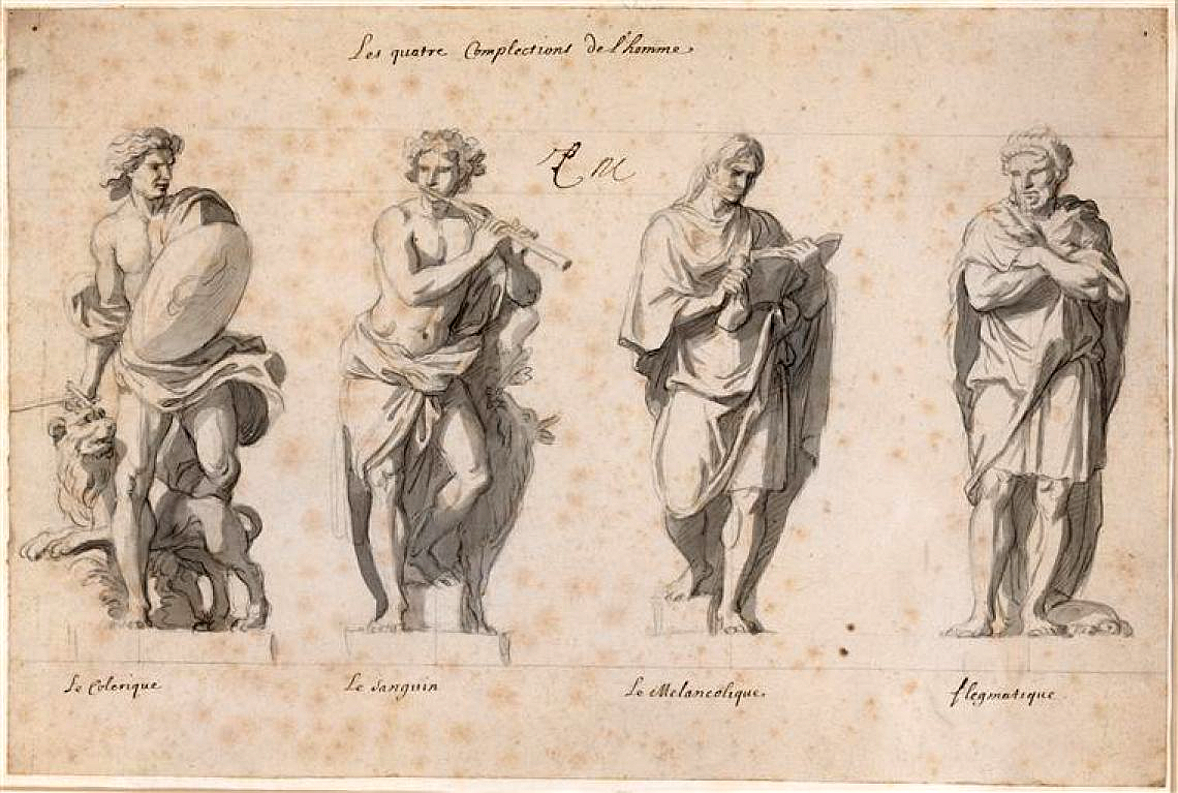
\includegraphics[width=1\textwidth]{temperaments}
  \centering
  \caption{The four temperaments by Charles Le Brun, part of the \emph{Grande Commande}. Source: Wikimedia Commons Public Domain.}\label{fig:temperaments}
\end{figure}

% Darwin
Charles Darwin first described the importance of emotions in communication, and their relevance across cultures and even species. In his book ' \emph{The Expression of the Emotions in Man and Animals} ' he writes ' \ldots the young and the old of widely different races, both with man and animals, express the same state of mind by the same movements.' ~\cite{darwin1872emotions} He noticed that surprise was shown in humans across cultures, and even some mammals by raising the eyebrows. By framing emotions as a mean of communication, Darwin enabled the study of expression, and understanding of emotions as an evolutive advantage.

\begin{figure}[H]
  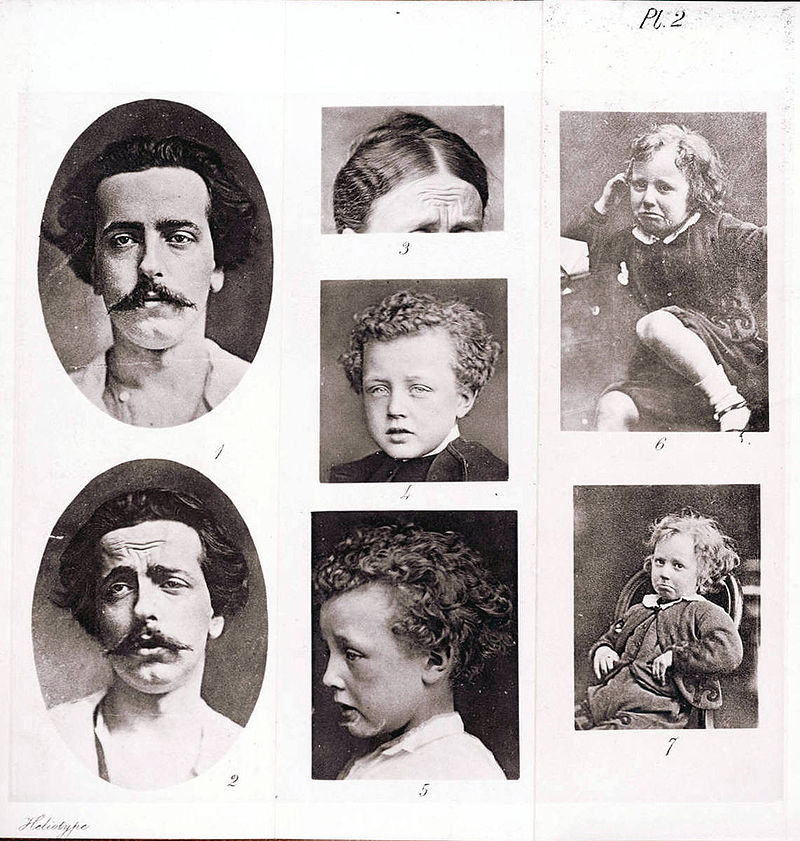
\includegraphics[width=1\textwidth]{darwin}
  \centering
  \caption{Illustration of grief from Darwin's \emph{"The Expression of the Emotions in Man and Animals"}. Source: Wikimedia Commons Public Domain}\label{fig:darwin}
\end{figure}

% Ekman
Although Emotions were thought to be universal there was no measurement of it. The universality of emotions was first formalized by Paul Ekman in his 1997 paper: "Universal facial expressions of emotion". Ekman studied facial anatomy, and expressions of different populations and cultures across the globe. He arrived to the conclusion that there are seven universal facial expressions of emotion~\cite{ekman1997universal}.

\begin{figure}[H]
  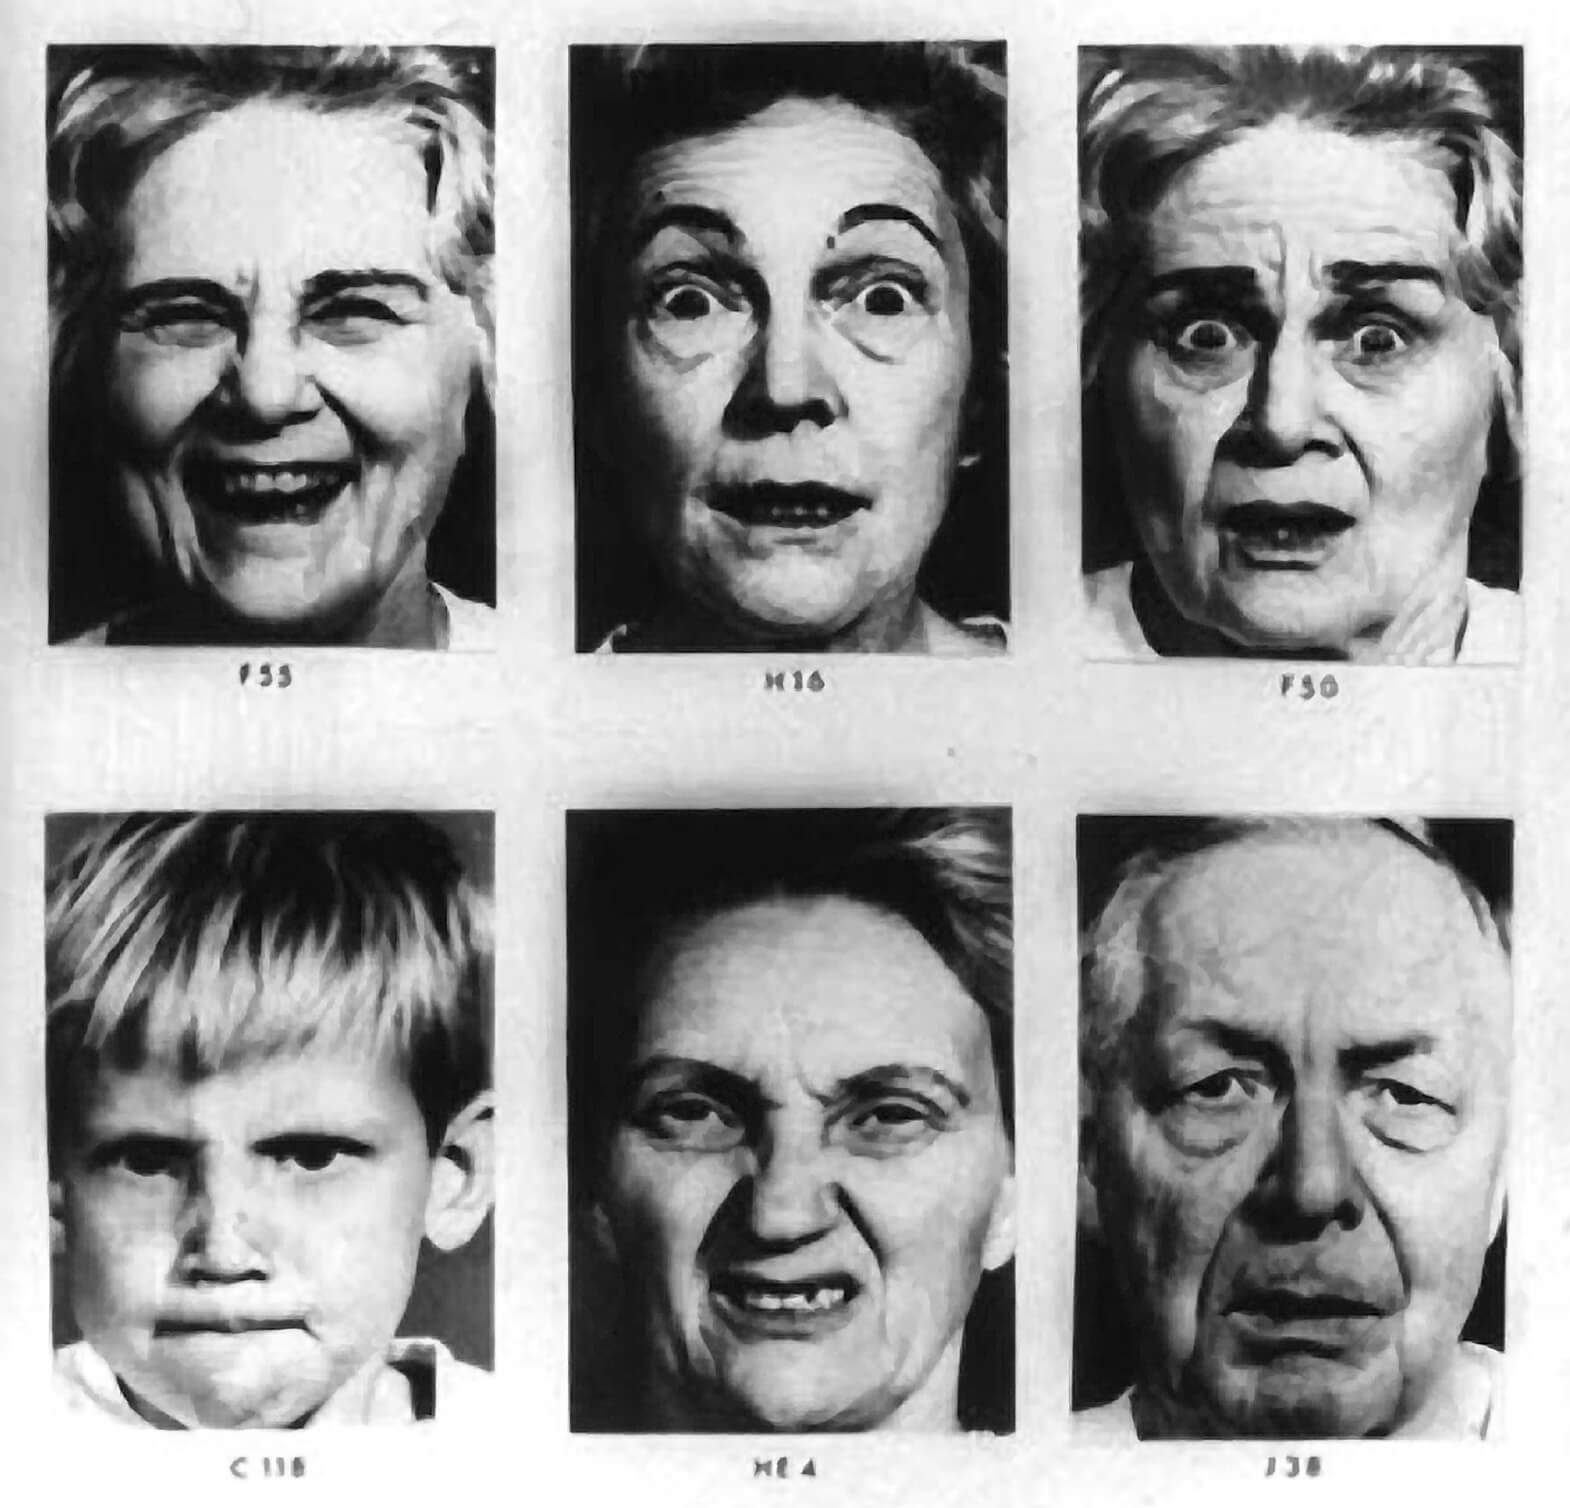
\includegraphics[width=1\textwidth]{ekman}
  \centering
  \caption{Ekman's photographs for cross-cultural research~\cite{ekman1999facial}.}\label{fig:ekman}
\end{figure}

% Picard
While emotions are a human concept, the digital advances of the millennium caught up and integrated with the field, to create the Affective Computing. The concept was first coined by Rosalind Picard, who not only created it, but is also a lead researcher in the field~\cite{picard2000affective}. The concept was originally related to Human-Computer interactions, and had the goal of computers expressing and recognizing emotions.

% Plutchik
Concerned with the subjectivity of emotion measurement, and the lack of generalization of self-report affect scales, Robert Plutchik proposed a method of measuring the basic emotions in a systematic way. He also proposed a way of deriving new emotions from the universal set proposed by Ekman. This was to be done based on theory, with enough diversity, but systematically relatable to the universal emotions~\cite{plutchik2013measurement}. In this way, the Plutchik model of emotions was created. This model is based on Ekman's universal emotions. Today, most Machine Learning tasks and datasets use this model of emotions. Different models will be discussed further in this chapter.

% Feldman
It is important to consider that for the last two decades, emotions have been studied based on Ekman's work on universal emotions. Although these do provide a framework for understanding how emotions came to be a part of the human experience, they do very little for their definition, or the description of emotions in language. Humans are complex, and even the most reliable model of universal emotions has exceptions. Psychologists interpret those differences with the help of the Theory of Constructed Emotions. This was first published by Lisa Feldman in 2014, and it describes the phenomenon of human emotions as a two-sided event: Affect and Emotion. Affect is a physiological phenomenon, the almost mechanical process that will enable behavioural response. The Emotional response is the cognitive contextualization of the former~\cite{feldman2014constructed}. Separation of physiological and cognitive responses allows the explanation of both, universality, and individual subjectivity.


% Worrying Definition of emotion
\subsection{Definition of Emotion}\label{sub:Definition of Emotion}
Within the context of this project it is important to distinguish between emotion and affect. Affect, in the context of this project will be treated as a term to associate predisposition towards stimuli. Thus, affect is in a sense, a general term that can be even used to describe animal, and other non-human entities. Emotions, on the other hand, are treated in this project as a state inherent to humans. This state is multidimensional, and every dimension, or emotion, can either be present in a certain amount, or not be present at all.
Emotions present an affect value, but not necessarily otherwise.


% DELIMITATION

\subsection{Affect}\label{sub:Affect}
In the context of this project the term Affect will be used to denote the autonomous physiological response of the human body to external stimuli, as well as the measure of these in terms of Valence, or Arousal. This definition complies with the Theory of Constructed Emotions, without invalidating the extended use of affect models of language.

The relevance of affect in text has increased since the popularization of text-based social networks, like twitter. There, individuals and organizations openly express their opinions. This creates an environment where implicit feedback about entities is present. An easy way to abstract popular opinion about a named entity is learning the affect expressed in text, such as a tweet. Affect can be a multidimensional phenomenon, but the most important dimension of it is valence: whether a text expresses positive or negative affect. This use of affect language models has proven useful to marketing, public relationship, and social sensing, but does not provide an insight into the human experience of emotion further than a single dichotomical variable.

Affect is relevant to this project since emotions can be represented within the models of affect that include valence and arousal~\cite{barradas2016thesis}.

\subsection{Emotions in Communication}\label{sub:Emotions in Communication}
According to darwin, the main evolutive advantage of emotions is to be able to communicate an internal state with others~\cite{darwin1872emotions}. The communication, and therefore, the detection of emotions can be done through three different means:
\begin{itemize}
  \item \textbf{Language or self report}: Using language, verbal, written, or otherwise, to express content with emotion, or explicitly declare an emotional state.
  \item \textbf{Facial Expressions}: The activation of different sets of facial muscles to express emotion. This must be measured visually.
  \item \textbf{Bio-signals}: The change of physiological states usually related to the limbic system can be measured through bio-sensors. This more accurately represent affect, but emotions can be measured through it.
\end{itemize}

This project is focused on language expressions of emotion. More specifically on expressions of emotion through text. This means that this project will not directly measure emotions on humans, but on text written by humans. These represent the expression of a momentary emotional state, expressed through text, and stored for later analysis. Text analysis is a subset of the field of Natural Language Processing (NLP). This project is heavily based on NLP concepts. For this reason, different methods for emotion analysis in text are discussed next.

\subsection{Models of Emotions}\label{sub:Models of Emotions}
When searching for expressions of emotions in text, one must know what kind of emotions are being searched for. When asking a person what emotions do they know, a plethora of emotions can be named, but most of these are language, culture, or context dependent. Under certain cultures, or even sub-cultures, new emotion names can emerge, that describe a general emotion under different context. Considering the theory of constructed emotions, there is as many emotions as context there are. Fortunately, the study of emotions being done here is restricted to the communication of emotions. For the communication of emotions a consensus must be made.
A model of emotions is the selection and structure of categories in which the expression of an emotion can fall, commonly called 'Universal Emotions'. These are usually formed through the analysis of human (and some times animal) behaviour, with the framework of a theory of behaviour. In this section we introduce some relevant models of emotion for ML and NLP.

\subsubsection{Ekman's model of Emotions}\label{subs:Ekman's model of Emotions}
As mentioned in \ref{sub:Historic Milestones}, the most widely recognized model of universal emotions in humans was created by Paul Ekman\cite{ekman1992basic}. This was created through the observation of facial expressions. Facial expressions are measured through Activation Units (AU's): Sets of muscles that, when contracted, deform the figure of the human face in specific ways. Emotions are then characterized by the activation of different sets of AU's. The current model of universal emotions contains seven emotions:

\begin{itemize}
  \item Anger
  \item Disgust
  \item Fear
  \item Surprise
  \item Happiness
  \item Sadness
  \item Contempt
\end{itemize}

Although this model is based on facial expressions, most studies of emotion use this as the base model to explore and understand concepts of human behaviour. Notice that this model is based on the communication of emotions through facial expressions. These are said to be universal because facial expressions seem to have been forged through natural selection, and are independent of culture, language, or segregation of populations. In simple terms, humanity had a face for longer than most other human traits. Under this frame of reference, language as a mean of communication is a relatively new phenomenon, but since it allows for more detailed communication, it changes the way we communicate our internal states.

\subsubsection{Plutchik's model of Emotions}\label{subs:Plutchik's model of Emotions}
Although Ekman's model provides a firm base for universal emotions, it lacks structure. Robert Plutchik created his model by removing Contempt, and adding two more emotions: anticipation and trust. By doing so, a three-dimensional model was created that also provided dichotomical, or polar emotions, intensities, and derivatives through superposition.

\begin{figure}[H]
  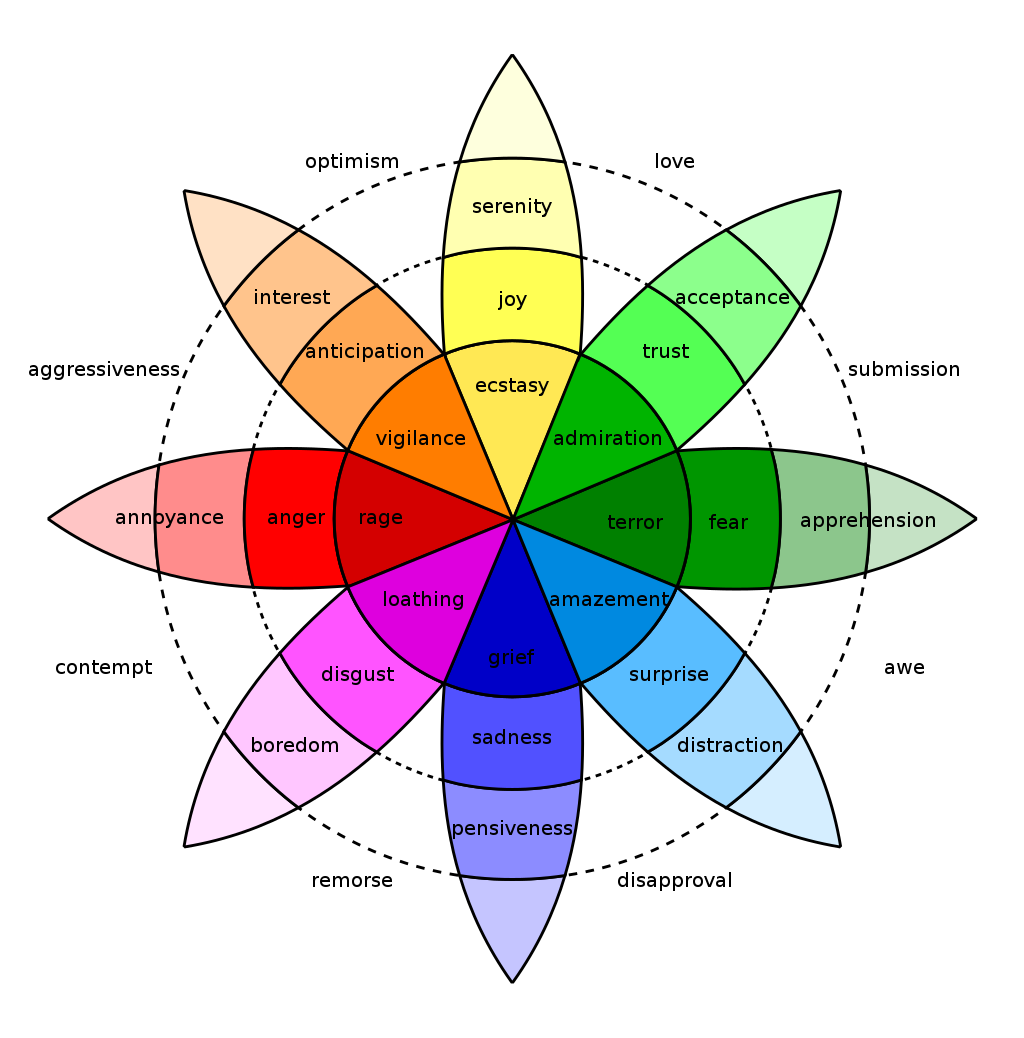
\includegraphics[width=1\textwidth]{plutchik}
  \centering
  \caption{Plutchik's wheel of emotions. Source: Wikimedia Commons Public Domain}\label{fig:plutchik}
\end{figure}

The model shown in Figure \ref{fig:plutchik} shows these characteristics. The main emotions are expressed in different intensities, and named accordingly. The combination, or superposition of some emotions receives a new name. This model is so well structured and colored, that it has called the attention of the scientific and engineering community. Unfortunately the premises of this model are faulty, and the scientific basis are questionable. The subjective nature of emotions doesn't allow for strict dichotomies. A simple poll asking 'What's the opposite of joy?' will turn in two answers: Anger and Sadness, depending on the context.

According to the theory of Constructed Emotions, it is exactly context that creates emotions. This means that culture, language, learning, and many other environmental factors contribute to the characterization of an emotion. For this reason, when studying emotions in text, a mean of contextualizing an emotion word is necessary.

\subsection{Emotions and Text}\label{sub:Emotions and Text}
When it comes to contextualizing words, linguists have had tools since the 1930's~\cite{corson1996fields}. This is the case of Lexical Fields. In it's simplest version, this tools ask people what words are most closely related to a concept. The result of a free association can be a network of interrelated words, or a set of words that relate to a concept. This set is also called a semantic field.
By asking people what emotions are related to a specific word, a semantic field of emotions can be created.

This is exactly what Saif Mohammad did in 2013~\cite{mohammad2013crowdsourcing}, creating the Canadian National Research Council Emotional Lexicon (NRC EmoLex). This contains around 14 thousand words, and their association with the 8 basic emotions of the Plutchik emotion model. This was an incredible effort, since several people must review every single word and emotion relationship, and evaluate them.
All this work can actually be inferred from large corpus. By creating a network of word relationships, WordNet provides a way to cluster into affective words~\cite{strapparava2004wordnet}. This proves that a representation of emotions in text can be learned from text, without human intervention. Machine Learning provides tools to optimize this representations.

\section{Emotion and Machine Learning}\label{sec:Emotion and Machine Learning}
The field of Natural Language Processing has seen great advances in recent years thanks to the use of Machine Learning for automatic inference of language models.

While there are many ways of using ML within NLP, the methodology this project focuses on is Word and Sentence Embedding. Embedding is the process of giving a numeric representation to a word or sentence within a corpus. This allows for computational models to easily manipulate text data that would otherwise be an arbitrary encoding of text. With the advances in machine learning automatic word embedding became a possible solution to avoid crowdsourcing.

Several machine learning approaches try to automatically learn the best numeric representation for characters, words, or sentences given the context of a dataset. In the last decade there have been many efforts from research groups to generalize these embeddings though the use of powerful models, and bigger datasets.

% Word2Vec
One of the first models to call the community's attention was Google's Word2Vec\cite{mikolov2013word2vec}. A model trained on news articles that allowed for complex language representation, like lexical arithmetic. This model has the model of an Autoencoder, and is therefore unsupervised.
% Should I talk more about dimensionality reduction/ autoencoders?

After Word2Vec, a series of language models were created. Word2Vec successors include ELMo, GloVe, which are similar but consider more or different context when creating the language model. With the creation of the transformer in ML~\cite{vaswani2017transformer}, a second wave of ML language models were created. XLM, GPT, BERT and it's many iterations, all provide a language model that captures not only the representation of a word, but also it's context.

These models learn to represent words from context: By looking at the words and sentences in a document, a contextualization is given to the use of a specific word, in every document. These language representations are far from a lexicon. They are numerical representations that, due to their automatically learned creation, are difficult for humans to interpret. Once these models are trained on large amounts of data, the trained model can be stored, and re-distributed to be used in different language tasks. This is called a pre-trained model. For this reason, such a context-dependent model can be used in short sentences, or even single words: The model is in itself the abstraction of a large amount of language data, learned through text documents.
There exist also models trained not on documents, but on dialogues. These models will not be used in the context of this project.

By observing the abstract representations of these models, one can learn how specific concepts are learned by pre-trained ML models from text.

\section{Problem setting}\label{sec:Problem setting}

Given pre-trained language models, and corpus of labeled text with single emotions, can we find the similarity between the structure of the representation of said text and their emotions in the abstract space created by the language model and a model of emotions backed up by scientific research?

\section{Objective}\label{sec:Objective}

To quantifiably and objectively analyze the representation of emotions in Machine Learning pre-trained Language Models, while presenting a human-understandable qualitative description to promote the discussion of models of emotions and automatic learning of human concepts in Natural Language Processing, and Machine Learning.

As consequence of this objective, the methodology to analyze a dataset of labeled emotions based on pre-trained language models is to be established. The intuitions and qualitative results of this project are to be developed into actual analysis methods to be used in the understanding of language models.


\section{Justification}\label{sec:Justification}
Be it in dialogue, local or international media, or even entertainment, current events have proven that the incorrect understanding of the emotional response of the general population can lead to severe social problems. Subcultures, minorities, and oppressed populations are expressing their problems and difficulties in platforms all around the internet. People need to express themselves,be heard and understood, as well as understand other points of view, but untrained emotional reaction is being weaponized to discourage discussion, dialogue, and democracy. Be it as a political or military action, or simply by lack of self consciousness, the emotions of every technology user and media consumer can turn against themselves. Justified pacific protests can turn into meaningless riots. Rational arguments can turn into senseless discussions, that separate populations and capture us in our subjective realities. I believe that the understanding, awareness, and acceptance of our emotions and others' can lead towards the path to dialogue, comprehension and peace. To do so at a scale as large as the one presented by the internet, and global media, we must use the same tools that have created such a vast field. The understanding of our data, ML and AI models, and their representations of our reality can help us understand ourselves. This project is at it's core, an attempt at understanding human nature.

 %!TEX root = ../thesis.tex
\chapter{Related Work}\label{chap:Related Work}

% TODO write after introduction

\section{Lexicons}\label{sec:Lexicons}

Mohamad and Turney created an Emotion Lexicon through crowdsourcing~\cite{mohammad_crowdsourcing_2013}. In this way an emotional word embedding was created by subjectively asking participants whether or not a word was related to a specific emotion.

\section{Automatic Approaches}\label{sec:Automatic Approaches}
Vo and Zhang created an automatic approach to learning sentiment lexicons for short texts through the use of emojis~\cite{vo_dont_2016}. This method uses the intrinsic usage of emojis to express positive or negative valence in a sentence, and exploded this to expand that valence to words used in the same context.

Maas et al\. created a method to learn word vectors for sentiment analysis~\cite{maas_learning_2011}.

By applying machine learned automatic embeddings, the creation of word embeddings based only on text data was open as a possibility. This is also a method that later became the popular Word2Vec method~\cite{mikolov_distributed_2013}.

A refining of word embeddings has been suggested by Yu et al\. by means of a clustering algorithm on the vector space~\cite{yu_refining_2017}.

Rothe et al\. suggested an orthogonal transformation to word embeddings used on SemEval2015 which yielded ultradense word embeddings for affect~\cite{rothe_ultradense_2016}.

A further exploration of transformations of a word vector space was done by Hollis et al\. by means of component analysis, thus creating models of semantics from text. These were applied to affect\cite{hollis_principals_2016}.

These studies have mostly been done with affect: positive and negative valences, but have mostly ignored other emotional dimensions.

\section{Word Embeddings}\label{sec:Word Embeddings}


\section{Language Models}\label{sec:Language Models}
There is an incredible amount of pre-trained Machine Learned Language models. For this project we have selected models based on the following criteria:

\begin{itemize}
  \item The model was trained with a large amount of general purpose language corpora.
  \item It represented a breakthrough in NLP tasks at the moment of its publication.
  \item The model has been reproduced, implemented, and tested in many ML language tasks.
\end{itemize}

Under this criteria, four models have been spotted as candidates for the experiment:
\begin{itemize}
  \item Word2Vec: Words to Vectors
  \item GloVe: Global Vectors for Word Representation
  \item ELMo: Embeddings from Language Models
  \item BERT: Bidirectional Encoder Representations from Transformers
\end{itemize}

Word2Vec is the result of converting large corpus into itself, by using an auto-encoder method, with help of a one-hot encoding of the corpus vocabulary~\cite{TODO}. At the time of its publication it captured much atention, mostly due to the posibility of semantic artimetic. This was tipified by the \"King - Man + Woman = Queen\" example. Due to the one-hot encoding step in the algorithm, it does not solve the problem of words with multiple meanings.

Glove is recognizable between other language models, for its linear substructures of meaning. Since it was trained on aggregated co-occurrence statistics, it captures semantic structure better than Word2Vec~\cite{TODO}. It still asigns a one-to-one representation of words and embedded vectors, so it does not solve ambiguities.

ELMo solved this last mentioned problem by analyzing context\cite{TODO}. This was acheived by training on prediction of words in forwards and backwards passes. Even though this model solved the problem of context-dependant meaning, it was created with the premise that context in text is secuential, and it's architecture dependant on LSTMs showed this.

BERT was the first algorithm to solve this problem, by implementing a context-dependant learning, that is not based on the secuential structures. This was done with the use of Transformers. A deep learning architecture based on the atention model, that does not depend on secuential structures.

Both BERT and ELMo give different embeddings to words in different contexts, but BERT has proven better at solving language tasks. For this reason, only BERT will be used in this project.

One last model will be used as a mean of comparing results between the different models. This is FastText \cite{TODO}. FastText is very similar to the algorithm with which word2vec was created. It creates a one hot encoding of a corpus, and creates a latent dimension through training either an autoencoder, for an unsupervised approach, or a classifier, for a supervised one. This algorithm requires traning on the corpus. Since the corpus selected on this project are relatively small, FastText provides a way to create a baseline for pretrained models, by analyzing what a basic model trained only on the corpus would look like.

\subsection{Selected Language Models}\label{sub:Selected Language Models}

Considering the prospective models, and the given criteria, the selected models for embedding the datasets are the following:
\begin{itemize}
  \item Fasttext
  \item Word2Vec
  \item GloVe
  \item BERT
\end{itemize}

\subsubsection{FastText}\label{subs:FastText}
Python's FastText library\cite{TODO} is used in this project. This provides two approaches for training the model: an unsupervised, and a supervised. The unsupervised requires a text file with one sentence per line. The algorithm is in charge of the tokenization. This of course only works in english. The supervised approach requires a similar file for the corpus, but at the end of every line, two underscores most be followed by the label of the given sentence.

\subsubsection{Word2Vec}\label{subs:Word2Vec}
Since this pre-trained model has a one-to-one correspondance between word and embedding, a dictionary can be downloaded and imported via the gensim python library~\cite{TODO}. This model has been trained with the Google News \cite{} corpus. It weights about 1.5 Gb, and has a latent space of 300 dimensions. It is supposed to be located at the url \url{https://code.google.com/archive/p/word2vec/}, but the file is not to be found. Forums on google groups for the word2vec (\url{https://groups.google.com/forum/#!topic/word2vec-toolkit/z0Aw5powUco}) point several urls where the model can be found.

\subsubsection{GloVe}\label{subs:GloVe}
This model, provided by the Standford University, is of easy access, and as Word2Vec, can be imported as a dictionary \cite{TODO}. The download can be found under \url{https://nlp.stanford.edu/projects/glove/}. This specific version selected was trained on the Wikipedia corpus, contains 6 billion words, uses 300 latent dimensions, and weights less than 1Gb.

\subsubsection{BERT}\label{subs:BERT}
The BERT model is trained not with one, but two types of tasks. The first one is masked word or sentence prediction, and a second one requires extra layers on the architecture and a fine-tunning training for task specific performance. \cite{TODO} The pre-trained model that one can get is the language model trained with the masked-language task. This model is not as easy to get, since the defoult python libraries to import BERT, require training and fine-tunning. For this reason, the bert-embeddings python library has been selected for this task.

\section{Analysis Algorithms}\label{sec:Analysis Algorithms}
Two algorithms have been chosen for dimensionality reduction:
\begin{itemize}
  \item PCA
  \item TSNE
\end{itemize}

PCA can be interpreted as a linear transformation on the input space, that yields the maximum explainability by the least amount of dimensions. While TSNE uses statistical information to maximize the distribution of information of groups, while minimizing the distribution of information within groups.

\section{Datasets}\label{sec:Datasets}
There are many datasets of \"emotion in text\" on the internet, and finding them is not a new problem. Unfortunately, the methodology and rigor for their creation cannot be easily tested. A heavy use of the paper "An analysis of annotated corpora for emotion classification in text" by Klinger in 2018 \cite{klinger2018analysis} was done. This paper not only collects information about the datasets, but also tests their valididty in the context of a text cliassifier.

\subsection{Inclusion Criteria}\label{sub:Inclusion Criteria}
To be included into these experiments, the following criteria must be met by a dataset:
\begin{itemize}
  \item The dataset must contain short labeled texts, in english.
  \item The label must be a single emotion, from an eckman-analogous emotional model.
  \item The labels must not be a reference to valence, arousal, dominance, or other affect models.
\end{itemize}
% Justification
The text to be analyzed must be in english, since the methods and language models that we are testing will not all be available in other languages. The single-single label criterion has been chosen due to the restriction of two-dimensional projections, and their visualizations as scatter plots. The label is to be exrpessed as a single color on scatter plots, and a multi-label problem would not present the effect desired  when developing the desired intuitions.

\subsection{Candidate datasets}\label{sub:Candidate datasets}
For the datasets included in Klinger's original paper~\cite{klinger2018analysis} the naming in the paper was not followed. This is due to the inconsistencies between the paper and their github repository, which (as the moment of writing this thesis) was last updated on Dec 17 2019 (commit e58d676). The dataset naming conventions used here is the same as in the document called "unified dataset of emotion in text": \url{https://github.com/sarnthil/unify-emotion-datasets/tree/master/datasets}.

Lastly, the candidate list includes the datasets mentioned, but is not restricted to them:
\begin{itemize}
  \item AffectiveText~\cite{strapparava2007semeval} % VAD
  \item AIT-2018~\cite{SemEval2018Task1} % VAD
  \item CrowdFlower % USED
  \item DailyDialogs~\cite{li2017dailydialog} %TODO: might need to be included
  \item Emotion-Cause~\cite{ghazi2015detecting} %TODO: might need to be included
  \item Emotiondata-Aman~\cite{aman2007recognizing} % VAD
  \item EmotionPush~\cite{huang2018emotionpush} % USED
  \item EmoBank~\cite{buechel2017emobank} % VAD
  \item fb-valence-arousal~\cite{preoctiuc2016modelling} % VAD
  \item Friends~\cite{chen2018emotionlines} % USED
  \item Grounded-Emotions~\cite{liu2017grounded} % I seriously don't know what's up with this ds
  \item ISEAR International Survey On Emotion Antecedents And Reactions~\cite{scherer1990international} % Format not open source
  \item Tales~\cite{alm2005emotions} % Two different annotators, two different labels.
  \item EmoInt \cite{MohammadB17starsem} %TODO: might need to be included
  \item TEC The Twitter Emotion Corpus published \cite{mohammad2012emotional} %TODO: might need to be included
  \item Electoral-Tweets \cite{mohammad2014semantic} %TODO: might need to be included
  \item SSEC The Stance Sentiment Emotion Corpus published \cite{schuff2017annotation} %TODO: might need to be included
\end{itemize}
The link to these datasets can be found under the github repository for the unified emotion datasets.
https://github.com/sarnthil/unify-emotion-datasets/tree/master/datasets
From this list, several datasets use an affective model of valence, arousal or dominance. Removing the datasets that do not explicitly comply with the inclusion criteria leaves the following:

\begin{itemize}
  \item CrowdFlower % USED
  \item DailyDialogs~\cite{li2017dailydialog} %TODO: might need to be included
  \item Emotion-Cause~\cite{ghazi2015detecting} %TODO: might need to be included
  \item fb-valence-arousal~\cite{preoctiuc2016modelling} % USED
  \item Friends~\cite{chen2018emotionlines} % USED
  \item EmoInt \cite{MohammadB17starsem} %TODO: might need to be included
  \item TEC The Twitter Emotion Corpus published \cite{mohammad2012emotional} %TODO: might need to be included
  \item Electoral-Tweets \cite{mohammad2014semantic} %TODO: might need to be included
  \item SSEC The Stance Sentiment Emotion Corpus published \cite{schuff2017annotation} %TODO: might need to be included
\end{itemize}

% What datasets were selected and why?
During the exploratory phase of this project, a subset of these datasets will be selected, giving priority to those with a more standardized, cleaner, or easier to access data.
Models

\section{Research Question}\label{sec:Research Question}

As a general research question we propose to answer the following:
When using pre-trained models for word and sentence embedding, \textbf{is the information about the emotional and affective content or context of the word or sentence represented in the vector space?}

This question can be approached in three different ways:
\begin{itemize}
  \item Is there a direct correlation between any of the dimensions of the vector space and human-labeled emotions and affect?
  \item Is there a linear transformation that will yield a direct correlation to the same human-labeled emotions?
  \item Is there a hierarchical structure that accurately represents the embedding of said labels?
\end{itemize}

 %!TEX root = ../thesis.tex
\chapter{Methodology}\label{chap:Methodology}
% Justification for the methodology

To analyze the representation of emotions in different word embeddings, a high emphasis on dimensionality-reducing visualizations was done.

The steps to do so are the following:
\begin{enumerate}
  \item First, the selected datasets must be embedded in their vector space. This will allow for a faster processing of the data, but requires making the technical decision of how the word vectors will be turned into sentence vectors to share the label in the case of datasets that contain a label for every sentence.
  \item A supervised clustering must yield accuracy similar to that of a classification task. This means testing the accuracy of a classifier on the emotion recognition task. Even though this step could be seen as optional, failing to reproduce the baseline accuracy scores for this simple task might mean that the embeddings are not even capturing the basic information about the task.
  \item A correlational analysis will be done between every dimension of the vector space and the emotions present in the dataset. This will tell us about any linear representation of emotions in the vector space.
  \item A second study must show if a linear transformation of the vector space dimensions will yield a better correlation with the emotions of the datasets. This means either LDA, or PCA\@.
  \item A hierarchical clustering will be used to analyze any possible structure in the embedded dataset in relation to emotions.
  \item A final approach to this problem can be done through the study of oppositeness.
\end{enumerate}

The mentioned methodology is based on answering the research question with progressive approximations. It is highly unlikely that a simple embedding model represents emotions in a single dimension in a linear manner, but it is increasingly more likely that some correlation is found with a linear transformation of the aforementioned. In case these two approaches present no information about emotions, a hierarchical clustering can extract the intrinsic information of affect in emotions. Since previous works have already shown that affect can be represented in vector spaces, created with a linear transformation of word embeddings\cite{TODO}, it would be contradictory to not find a hierarchical structure of emotions in this last step.


\section{Preliminaries}\label{sec:Preliminaries}
% What are the preliminaries? Environmental setup, and embedding.
% Justify those preliminaries here
This research was managed as both, a research project, and a software development project.
As a setup for this project, two steps were taken. Setting up the physical and virtual environments for the experiments, and converging the different datasets and model embeddings into a single data source.

With scientific rigor, order, and reproducibility in mind, a git repository has been setup, where not only the working environment is provided, but also the history of the project  development.


\subsection{Environment Setup}\label{sub:Environment Setup}
\subsubsection{Organizational}\label{subs:Organizational}
The project planning was layed out throught three months: March, April and May of 2020. A total of twelve weeks were divided into four equal sprints, where the four main tasks in the project were equaly separated in time: Exploration and Preparation, Programming, Experiments, and Writing. The four sprints were described by tasks, further divided by sub-tasks. These were kept in track and followed me, and both Supervisors through the Asana application\cite{TODO}.

The repository is accessible through github: \url{TODO}

\subsubsection{Hardware}\label{subs:Hardware}
% The computer
This project was implemented and executed in my personal computer: A Manjaro Linux x86_64, with Kernel 5.6.11-1-MANJARO. The available CPU is an Intel i7-8700K (12) @ 5.000GHz, and the GPU is an NVIDIA GeForce GTX 1080 Ti. A total of 15937MB of RAM memory were available for experiments, as well as 16GB of swap disk. Although much of the technology available for these experiments is more than necesary, the execution of some BERT models is not possible with these technical specifications. This influenced the selection of the BERT model to be used, and played a big part in selecting a pre-embedding of models.

\subsubsection{Software}\label{subs:Software}
% The operating system
As mentioned, the development and execution were on a Linux Operating Systetm (OS). The Distribution used was Manjaro. This OS is a rolling release distribution, so the version used changed allong the development. This is one of the reasons why virtual development and execution environments were used: to keep reproductability, and ensure a stable testing. The only reason for this OS to be used is that it is my personal computer.
% The repo
As a Version Control System (VCS), git was added to the repository. This enables distributed access and historical revision for anyone trying to reproduce or supervise the project.
% The development environment
Several development tools were used. For text editing and script execution, Atom 1.46.0 \cite{TODO} was used. Within the Atom environment, community packages were used to simplify the workflow: Hydrogen 2.14.1 \cite{TODO}, for example, allows the execution of python code from within the text editor, and can even show output of the lines executed. A list of the used packages is provided in~ \ref{TODO}
For some exploratory analysis, Jupyter Notebooks \cite{TODO} were used. To run these, a specific virtual environment was created with Docker 19.03 \cite{TODO} and NVIDIA-Docker. A docker image for theses notebooks was created. The dockerfile of this image contains the libraries used for data exploration. The downloading of the BERT models ran in TensorFlow is also contained in this dockerfile. The description and an initialization script for the virtual container are included in the project folder called "TF".
% How was the day to day? Explain on atom and script running
While the notebooks provided were used for data exploration, and visualization. Most of the development was done on the text editor. For this, python virtual environments were created with the help of the \lstinline{virtualenv} and \lstinline{virtualenvwrapper} python libraries. For these, a "requirements.txt" file was provided with the libraries used, and their versions.
% The development environment
When developping, the desired virtualenvironment was activated. After this, the atom editor is open on the desired folder. By doing so, the Hydrogen library takes the virtual environment for the execution of the code in the project.
By developing in this way, the whole project is available from the folder view on Atom. Code can be executed, and tested on the run, as if it were a Jupyter notebook, but changes are inmediately integrated into the code repository.
% Justification
This specific development environment was seleted to avoid conflicts between Jupyter Notebooks, and the VCS. The explorations are stored as notebooks, but cannot really represent the development of the project.
% The programming language
The Python programming language was used for the programming of the current project. This is due to it's incredible flexibility, access to the main ML libraries, and the predisposition of the Wirtschaftsinformatik und Maschinelles Lernen Institut. Under Python's umbrella of libraries, several were specifically added to enable this study. A List of the used libraries is provided in the appendix~\ref{TODO}.

% The ML frameworks
Two main ML frameworks were selected for the current project: TensorFlow 2.1.0 \cite{TODO} (TF), and PyTorch 1.4.0 \cite{TODO} (Also called Torch, for simplicity.). TF was selected specifically for it's access to a pre-trained BERT library \cite{} for embedding sentences. This was very usefull, since, compared to the Transformers library \cite{TODO}, it must not be fine-tunned. TF confronts developers with two main compatibility issues:

\begin{itemize}
  \item The cuda library being used most be a specific version. Most TF libraries will only work under CUDA library 9.2. Some might run under 10.1, but not under 10.2. Since the development environment is a rolling release linux distribution, the latest version of libraries is provided. Installing multiple versions brings problems to the day-to-day usage. Since the environment is also my personal computer, a virtual environment with containers were used instead, and for these, NVIDIA-Docker.

  \item at the moment of the development of this project, TF is undergoing a major version change, from 1.x to 2.x. Many reference libraries, and all code I have creted, used, or studied in my masters is depricated. The techniques learned during my studies need to be updated, and in many cases, re-learned.
  This is not an uncommon problem in technology, but it opens the opportunity for changing the work framework.
\end{itemize}

For all ML programming requirements that did not use the pre-trained BERT library, PyTorch was used. Certain algorithms were not programmed, but simply integrated from their implementation on python:

\begin{itemize}
  \item FastText: This algorithm was not implemented. It's python library from the implementaiton of Facebook Research was used. \cite{TODO}
  \item MulticoreTSNE: The TSNE algorithm was not implemented. Since it has heavy requirements on hardware, its implementation using distributed computing was used. \cite{TODO}
  \item Normalize: The sklearn version of the normalization algorithm was used due to its optimization. \cite{TODO}
  \item PCA: SKlearn version was used. \cite{TODO}
  \item Tokenization: Part of the embedding pipeline requires the tokenization of the sentences. This was done with the Spacy library, and the "en_core_web_sm" model.\cite{TODO}
\end{itemize}


\subsection{The Datasets}\label{sub:The Datasets}

\subsubsection{Access}\label{subs:Access}
% Crowdflower
http://www.crowdflower.com/wp-content/uploads/2016/07/text_emotion.csv

% EmotionX

\subsubsection{Storage}\label{subs:Storage}
The datasets were downloaded and stored under the project folder "data". Since every dataset is provided in different format and under different folder structures, every dataset is simply stored inside a folder with it's name.
Under the datasets folder, every selected dataset is accompanied by folders with the embedding model used to embed the dataset. Thus every dataset folder has several subfolders. On these subfolders, a python script called "embed.py". This script varies for every model and dataset. In general terms, it extracts the text and label from the dataset, embeds the text into the desired model, and stores it in a "csv" file under the same folder.
The "csv" file is stored under the name "embedded.py", except for the FastText model. In this case, there are two embedding approaches, one supervised and one unsupervised. Thus the names of the FastText embedding files are "embeddings_supervised.csv", and "embeddings_unsupervised.csv". Every other script creates a single "csv" file called "embeddings.csv".

% Different dimensionality on the dataset embeddings
Since every model embedds text in different

Thie file structure of the embedded files allows for exploration and experimental scripts to access the embedded data of different datasets, by building a single string with the dataset and model selected. This string must be prepended by the "./data/" folder name, and appended with the "embeddings.csv" string to generate a path that creates accesibility to the different datasets via a python coma-sepparated-value library, such as the built in \lstinline{csv}, or Pandas \cite{TODO} and it's \lstinline{read_csv} function. This effectively create a data source to be used in a data pipeline. This approach was selected due to it's simplicity.

% Maybe subsubsections?
\subsubsection{Embedding}\label{subs:Embedding}
The comparisson of the representation of different language models in this project requires a convergence of many different techniques. For this reason it was chosen to embed the datasets into an intermediate format, to later use them in experiments.

The embedding of the datasets is comprised of 5 steps:

\begin{enumerate}
  \item Loading model, text, and labels.
  \item Tokenizing text.
  \item Embedding every token into the model latent space.
  \item Average the given embedded words.
  \item Store the average sentence embedding.
\end{enumerate}

Loading text, and labels was done with either the CSV\cite{TODO} or the JSON\cite{TODO} python library, depending on the format of the data.

Tokenizing was done with Spacy's "en_core_web_sm" model, which allows access to the tokens via an iterator on the model, and the sub-compontent "text". An small snippet showing this process is shown in~\ref{lst:spacy}. This snippet considers a model has been loaded as a dictionary on tokens.

\begin{lstlisting}[caption={Tokenizing with Spacy},label=lst:spacy,frame=single]
import spacy
nlp = spacy.load("en_core_web_sm")
for token in nlp("This is a sentence in English"):
  word_embedding = model[token.text]
\end{lstlisting}

Every token is embedded in this way, but some models might not contain some tokens. In this case, the token is simply skipped. Some tokens with relevant information can be lost with using pretrained models that don't contain the complete vocabulary of the dataset, but it is expected, that the information distribution converge to the real distribution when large number of samples are integrated. This problem is later discussed in relation to training a model from zero~\ref{TODO}.

Once every token has been embedded into the model's latent space. A simple average is done across the tokens, keeping the dimensionality of the vector representation, and effectively creating a sentence embedding, represented in the model's latent space. This technique was selected since it's the most common \cite{TODO} method for sentence representation. With this method, the secuential nature of the tokens in the sentence is lost, in favor of providing a constant sized sentence embedding to compare between methods and datasets.

Lastly, the sentence embeddings are stored along with the label information. For this, the CSV format was selected, due to it's interoperabiliy, and accessibility. The statistics library Pandas has an excellent csv reader, but the data can also be imported into spreadsheet software, other statistical software, or very quickl loaded on to python with the CSV library. Every CSV file contains a header on the first row. The header is composed by $N+1$ columns where $N$ is the number of latent dimensions in the model. The last column is the "Emotion" column, where the label is stored. The name of every column starts with the letter "d", and is followed by consecutive numbers.

Since every pre-trained model is different, there were specific requirements on loading the model and embedding the tokens:

\subsubsection{FastText}\label{subs:FastText}
As previously mentioned, the FastText algorithm is an exception in this project, since it is NOT a pretrained model. The model is trained based on the dataset given. This can be done in a supervised, or an unsupervised manner. Due to the two methods for the usage of the FastText python library, the process of embedding a dataset with it requires two extra text files one with a sentence per line, and a second one, which includes the label as the last word of every line, prepended by two underscores (\lstinline{__}).

In both ways of training, the language model is being trained specifically for the dataset vocabulary. For this reason, all tokens will be available in the model's vocabulary, resulting in the most complete language model. This is at the cost of representing only the topics on the dataset. This is therefore also not a general languge model.

\subsubsection{Word2Vec}\label{subs:Word2Vec}
Word2Vec is trained in a very similar way as fasttext. Therefore, the expected results are similar. Word2Vec is treated within the context of this experiments as the pre-trained equivalent of fast text. The same number of latent dimensions, and a similar training approach were used. In this case, if a word in the dataset is not contained in the Word2Vec model, it is droped, and its analysis won't be included in the results of this project. Word2Vec was trained with a very large corpus, it is therefore considered a general language model.

The pre-trained model has been stored under the project folder "./models/Word2Vec/GoogleNews-vectors-negative300.bin.gz". The gensim python library is used to load the model in binary format without having to decompress it. This model is loaded as a dictionary. An example of this is shown in snippet~\ref{lst:load_w2v} that considers an iterator over a tokenized sentence.

\begin{lstlisting}[caption={Loading Word2Vec},label=lst:load_w2v,frame=single]
import gensim
model = gensim.models.KeyedVectors.load_word2vec_format(model_path, binary=True)
for token in tokenized_sentence:
  word_embedding = model[token]
\end{lstlisting}

\subsubsection{GloVe}\label{subs:GloVe}
Pre-trained GloVe models can be downloaded from the official website \url{TODO}. This model was downloaded and stored under the project folder "./models/GloVe/glove.6B/glove.6B.300d.txt". The name of this file contains two numbers: 6B is the number of words that are represented in this model, while 300d is the number of latent dimensions used to represent the vocabulary. This model has been trained for 50, 100, 200, and 300 dimensions. Since a smaller number of dimensions represents a lesser capability for representing complex language concepts \cite{TODO}, the larger version of this model was selected. This also concides with the number of dimensions used in Word2Vec, which makes results easier to compare.

\subsubsection{BERT}\label{subs:BERT}
Although BERT is a pretrained model, it's original distribution is considered to be only partialy trained. On the original paper \cite{TODO}, a fine-tunning task-specific phase is mentioned, and generally required for the model to work best. This fine-tunning also presents a great infrastructure challenge, since some pre-trained BERT models simply wont fit into a personal computer's RAM.

For this reason, the pre-trained BERT embedding library \url{https://github.com/imgarylai/bert-embedding} was used. This library allows for a selection of the BERT model, and the embedding of the whole sentence, without tokenization. The result is a json-like dictionary in Python that contains both the original sentence and the embedded sentence.

To be able to run the embedding notebook, provided under the project folder "exploration/Embedding with bert.ipynb", the following requirements should be met:
\begin{itemize}
  \item Docker >=19.03
  \item NVIDIA Container Toolkit
  \item This Docker TF Image: `tensorflow/tensorflow:2.1.0-gpu-py3-jupyter`
\end{itemize}

On Linux, the a correct installation of the nvidia-docker environment would yield a successful run of the following command: \lstinline{docker run --gpus all --rm nvidia/cuda nvidia-smi}

To build the docker image for this project, one must open a terminal on the "TF" project folder and run the following docker instruction: \lstinline{docker build -t bert .} where bert is the name of the image to be created.
Once this image has been built, docker can create containers with it. So to run the container necessary for the BERT embedding, the following command is used inside the project folder: \lstinline{docker run --gpus all -p 8888:8888 -v $(pwd):/tf -it bert}.
This last command will run a docker container, based on the "tensorflow:2.1.0-gpu-py3-jupyter" image, connect it to the localhost port 8888, and integrate the project folder to the jupyter server running on the container.

%TODO an image of how it the jupyter notebook looks, maybe?

Docker is used to comply with the complex requirements of TensorFlow, CUDA, and the bert-embeddings.Once the Jupyter server is running, the notebook can be opened, and executed. The loading of the model is shown in the following snippet~\ref{lst:load_bert}:

\begin{lstlisting}[caption={Loading BERT},label=lst:load_bert,frame=single]
from bert_embedding import BertEmbedding
bert_embedding = BertEmbedding(model='bert_24_1024_16', dataset_name='book_corpus_wiki_en_cased')
\end{lstlisting}

Here, the selected model is shown. This is a model with 1024 latent dimensions, trained on the Wikipedia corpus, and with case sensitivity. This means that words lowercase and uppercase letters will be embedded differently.

Within the notebook, a function was created to embed the datasets. This receives three arguments: a list of the sentences, a list of the labels, and the name of the output file, as a string. The embedding function is shown here:

\begin{lstlisting}[caption={Embedding with BERT},label=lst:embed_bert,frame=single]
def embed_and_save(X, Y, outpath):
    E = np.array([np.mean(t[1], axis=0) for t in bert_embedding(X)])
    with open(outpath, 'w', newline='') as f:
        fieldnames = [f"d{i}" for i in range(len(E[0]))] + ['emotion']
        writer = csv.DictWriter(f, fieldnames=fieldnames)
        writer.writeheader()
        for e, l in zip(E, Y):
            writer.writerow(dict({f"d{i}": ei for i, ei in enumerate(e)}, **{'emotion': l}))"
\end{lstlisting}

Running the embeddings for the datasets reported the following data:

\begin{table}[H]
  \begin{tabular}{lllll}
  Dataset                          & User              & System    & Total        & Wall        \\
  \hline
  \multicolumn{1}{l|}{CrowdFlower} & user 3h 57min 7s  & 13min 11s & 4h 10min 18s & 1h 5min 33s \\
  \multicolumn{1}{l|}{EmotionPush} & user 1h 28min 35s & 5min 25s  & 1h 34min 1s &  24min 31s   \\
  \multicolumn{1}{l|}{Friends    } & user 1h 26min 40s & 5min 3s   & 1h 31min 44s & 24min 9s
  \end{tabular}
  \caption{Runtimes for embedding datasets with BERT}\label{tab:rt_BERT}
\end{table}

This is much less than the "several days" reported by classmates. This might be due to the use of pre-trained models, and not running back-propagation to fine-tune the language models.

While running the embeddings, almost no GPU memory was used. This signals that the library is actually not making use of the GPU resources available. This also might mean that the embedding of the datasets might be much faster if the correct hardware resources are used.

At the beginning of the Year 2020, the library seemed a reliable way of getting the embedding done quickly. It allowed for embedding of the complete datasets in matter of minutes. Since I had been warned BERT embeddings could take days, I saw this as a gread advantage, and kept the method. Unfortunately as of May 2020, this library has been depricated. It's unmantained, and has requirements that might only be achievable under very specific conditions. This will not be a problem for reproduction, as long as the library is still available, and the provided docker image is used.

\section{Analysis}\label{sec:Analysis}
\subsection{Correlational Analysis}\label{sub:Correlational Analysis}
\subsection{Linear Dimentionality Reduction}\label{sub:Linear Dimentionality Reduction}
\subsection{Non-Linear Dimentionality Reduction}\label{sub:Non-Linear Dimentionality Reduction}
\subsection{Clustering Analysis}\label{sub:Clustering Analysis}

\section{Experiments}\label{sec:Experiments}
\subsection{Emolex}\label{sub:Emolex}
\subsection{Selecting Emotions}\label{sub:Selecting Emotions}
\subsection{Class Inbalance}\label{sub:Class Inbalance}
\subsection{Valence}\label{sub:Valence}

 %!TEX root = ../thesis.tex
\chapter{Experiments}\label{chap:Experiments}
The amount of experiments, data and visualizations created in this project are more than a dedicated reader is comfortable reading in one single pass. For this reason, the experiments and results in this chapter first presented with a simple example, the EmoLex. This example will guide the reader through the methodology to analyze the datasets, and introduce the intuitions presented through simpler visualizations with less data. With this intuitions in mind, the results of the other datasets, and language models are presented. In this way, the EmoLex works not only as an introduction to the methodology and results, but also as a lax baseline.

\section{EmoLex}\label{sec:EmoLex}
As an introductory experiment, EmoLex has been embedded into the abstract vector representation of the GloVe language model. This model was selected due to its one-to-one relation between word and embedding, and it's context independence. This means that a word will get one single embedding no matter what other words appear next to it. This in comparison to BERT, where the embedding of a single word depends on the tokens, words, and sentences that come with it. The EmoLex has single words related to emotions, so it must be noted that this experiment and it's results relate to word embedding, and not sentence embedding.

\subsection{Correlational Analysis}
A correlational analysis answers the question of how much does every dimension of the language model relates to every emotion. The result of this model is a correlation matrix where every element of that matrix is a number between -1 and 1.
In the case of the EmoLex, abstracted into the GloVe language model, it is a $8x300$ matrix, where the rows correspond to the 8 emotions represented in the EmoLex. This matrix is visualized in Figure~\ref{fig:cor_emolex_GloVe}. The plot shown in this figure is called a clustermap. It was created with pythons Seaborn library, and consists of two parts:

The main part is the visualization of the matrix. In this visualization, every number of the matrix is given a color from a range of colors shown in the color bar. The range is automatically set from the maximum and minimum number in the matrix. This allows to see patterns in the relationships between the vector space dimensions and the emotions, if there are any.

The second visualization of this plot is the left dendrogram. A dendrogram is the visualization of a clustering structure. This clustering is done through a nearest neighbor algorithm, using euclidean distance.

A correlational plot is used here to analyze the deviation of the distribution of the representation of variables in the different dimensions of the vector space. In this case, there are 8 variables. A uniformly random distribution of the representation would yield a correlation of 0.125. Thus a correlation of  0.125 or lower is considered random. In our baseline reference by Hollis et al.~\cite{hollis2016principals}, where they analyzed 9 variables the minimum significant correlation reported was 0.35. This is more than three times the correlation of a uniformly random distribution: 0.111\underline{1}

\begin{figure}[H]
  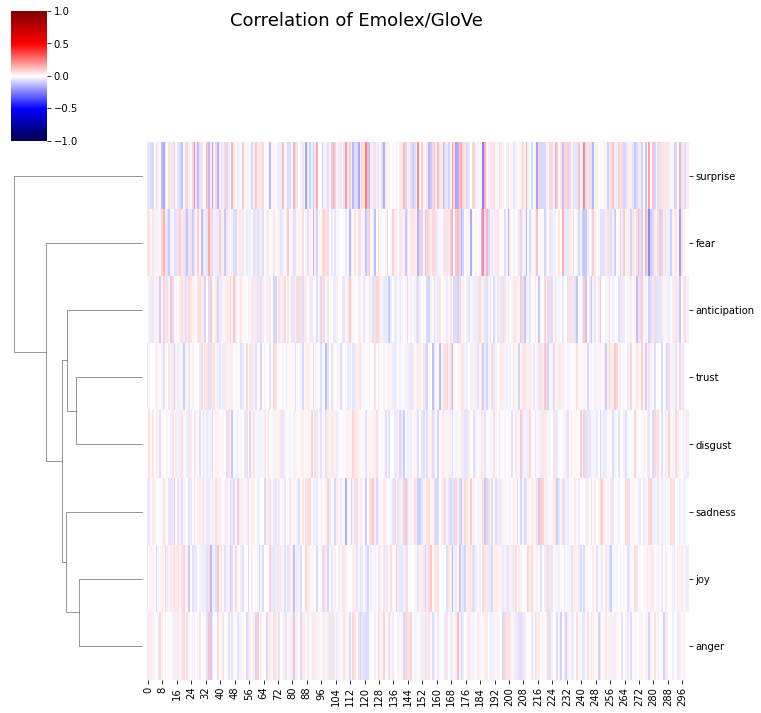
\includegraphics[width=\textwidth]{plots/emolex/cor_emolex_GloVe}
  \centering
  \caption{EmoLex Correlation Plot}
\end{figure}\label{fig:cor_emolex_GloVe}

In Figure~\ref{fig:cor_emolex_GloVe} it can be observed that represented by the GloVe model, the words contained in the EmoLex are uniformly distributed through the dimensions. The maximum correlation is 0.251, between the emotion 'Trust' and dimension 121 of the model. Although this is double the correlation that could be found thorough chance, it does not satisfy the baseline condition, and thus, we cannot consider that there is a linear correlation between the emotions of the EmoLex, and the dimensional representation of the Language Model.

The corresponding clustering algorithm shows that through their vectorial representation, the two most related emotions are joy and anger. This does not comply with the findings of dichotomical emotions, fitting into a valence model, as shown in the 2016 study~\cite{barradas2016thesis}.

These two results are enough to reject the hypothesis that there is a linear correlation between the emotions in the EmoLex and the vectorial representation of the GloVe model.


A further correlational study can be done solely to the labels of the EmoLex. This is here called an Emotion-to-Emotion correlation, and it's obtained through the self-correlation matrix of the one-hot-encoding of the EmoLex emotion labels. The clustermap of said matrix can be seen on Figure~\ref{fig:cor_emolex_GloVe_e_e}. An organic distribution of these would show the expected hierarchical clustering between positive and negative emotions. This plot, although labeled as related to the GloVe, is independent from the language model, since it only looks at the labels, but the name has been kept for consistency.

\begin{figure}[H]
  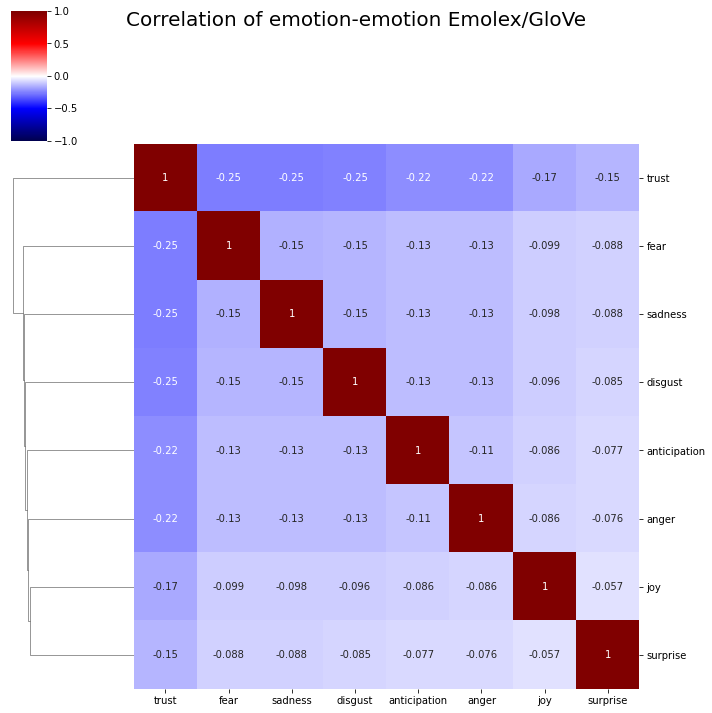
\includegraphics[width=1\textwidth]{plots/emolex/cor_emolex_GloVe_e_e}
  \centering
  \caption{EmoLex Correlation Plot}
\end{figure}\label{fig:cor_emolex_GloVe_e_e}

The EmoLex is not an organic corpus, and thus the labels do not represent the hierarchical clustering shown in the 2016 study~\cite{barradas2016thesis}. Instead the emotions are uniformly distributed. This is expected for a lexicon.

\subsection{PCA}
By maximizing the amount of information represented by the first components through a linear transformation of the data, a PCA analysis provides a perspective on the representation of variables in the model that cannot be seen through a simple correlation.

By visualizing a scatter plot of the first components or PCA dimensions, if there is a linear separation between the labels it can be visualized. Even in the case of data that is not linearly separable, a gradient of the distribution of the data could indicate the existence of a structure.

\begin{figure}[H]
  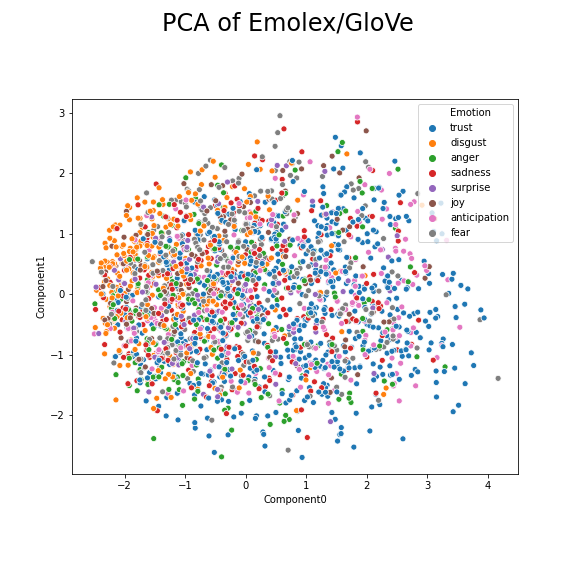
\includegraphics[width=1\textwidth]{plots/emolex/pca_scat_emolex_glove}
  \centering
  \caption{EmoLex Scatter plot of PCA}
\end{figure}\label{fig:pca_scat_emolex_glove}

In Figure~\ref{fig:pca_scat_emolex_glove} we can see the scatter plot of the words of the EmoLex, projected on to the first two components of the PCA transformation. Here we can observe, that the words labeled with the emotion disgust are mostly centered to the top-left of the plot. Although this might seem like the indication of a structure, we cannot certainly point at it. This plot is useful for visualizing linear separation, but that linear separation does not show in this case. To be able to visualize what the PCA transformation does to the vector space, the correlation matrix is shown next.

The correlation matrix shown next is the same type of visualization as the one in Figure~\ref{fig:cor_emolex_GloVe}, but this is done to the transformed dataset. This means that the x-axis shows the number of the component instead of the dimension of the language model.

\begin{figure}[H]
  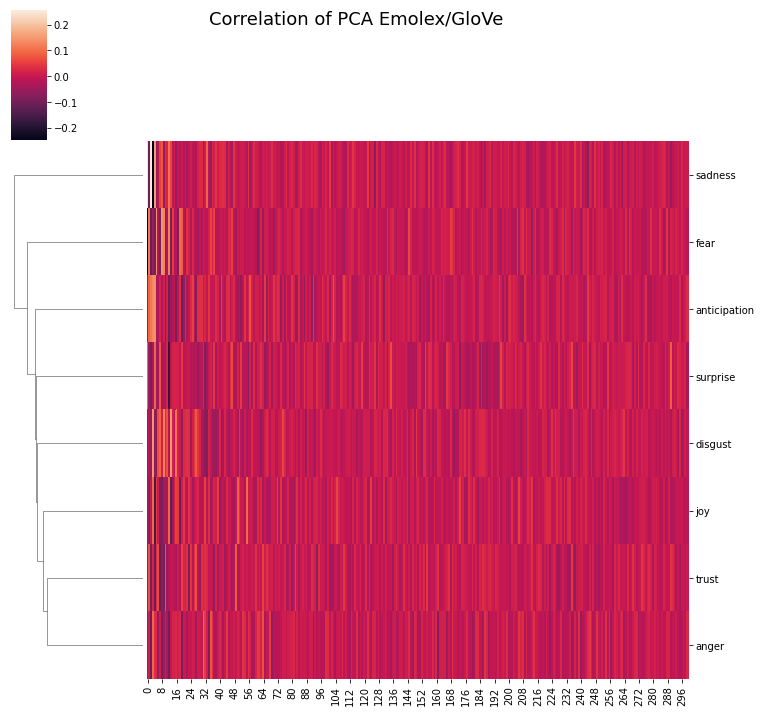
\includegraphics[width=1\textwidth]{plots/emolex/pca_cor_emolex_glove}
  \centering
  \caption{EmoLex Correlation of all PCA components}
\end{figure}\label{fig:pca_cor_emolex_glove}

By plotting the correlation matrix of the PCA transformation of the EmoLex, we can observe that most of the variability is concentrated on the first components. Still in this case, the maximum correlation is 0.2567, barely higher than on the linear correlation. The hierarchical clustering shows no presence of a valence-correspondent clustering.

Considering that the PCA is a linear transformation we do not expect to see better correlations between the model dimensions, and the concepts, but a dense representation that does not require looking at all dimensions. For this reason, when looking at PCA correlations, only the first eight dimensions will be shown. Eight is an arbitrary number that allows a square correlation matrix, since it's the same number of emotions for this dataset.

\begin{figure}[H]
  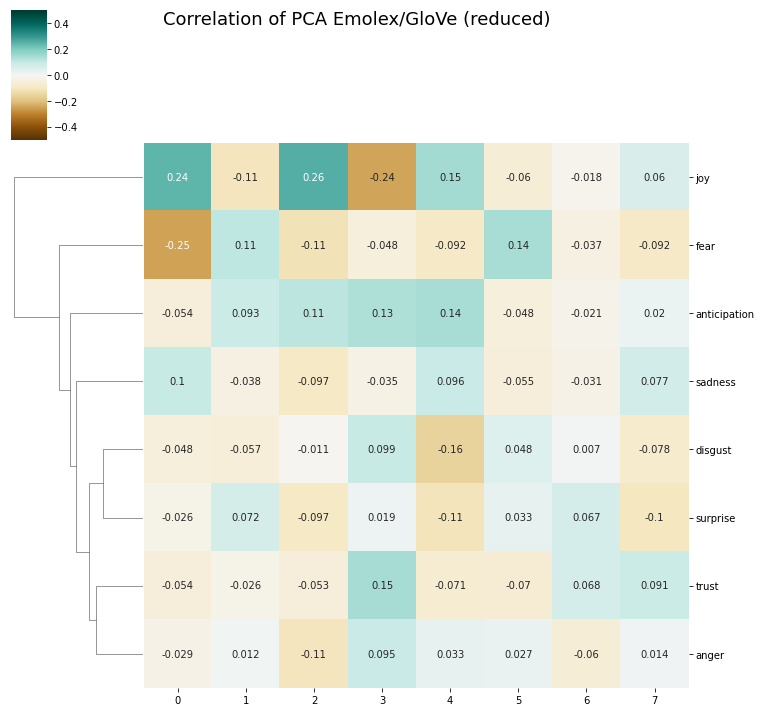
\includegraphics[width=1\textwidth]{plots/emolex/pca_cor_emolex_glove_min}
  \centering
  \caption{EmoLex Correlation of first PCA components}
\end{figure}\label{fig:pca_cor_emolex_glove_min}

Figure~\ref{fig:pca_cor_emolex_glove_min} shows the first 8 dimensions of the PCA transformation for this model and dataset. A different color scheme has been selected to easily identify between the linear correlation visualization, and the PCA-transformed correlations. This is the exact same data as the one used to create Figure~\ref{fig:pca_cor_emolex_glove}, but since only the most information-dense dimensions are being shown, the hierarchical clustering is much different. Here we can observe that what had no apparent structure now seems to cluster disgust with surprise, and trust with anger. By observing only the first component, we can see that if it activates, we can expect that the emotion Joy is not expressed in the embedding, with a 24\% probability, and that fear is not expressed with 25\% probability. This results are not very concise, but this is expected due to the artificial nature of the dataset, and the subjectivity of the concepts. In the experiments section of this chapter we aim at describing how much of that variability is due to the subjectivity of the concept.

\subsection{TSNE}
Through this, non-linear visualization algorithm we can plot a scatter that will concentrate the maximum variability possible on two dimensions. The result is the plot on Figure~\ref{fig:tsne_scat_emolex_glove}.

\begin{figure}[H]
  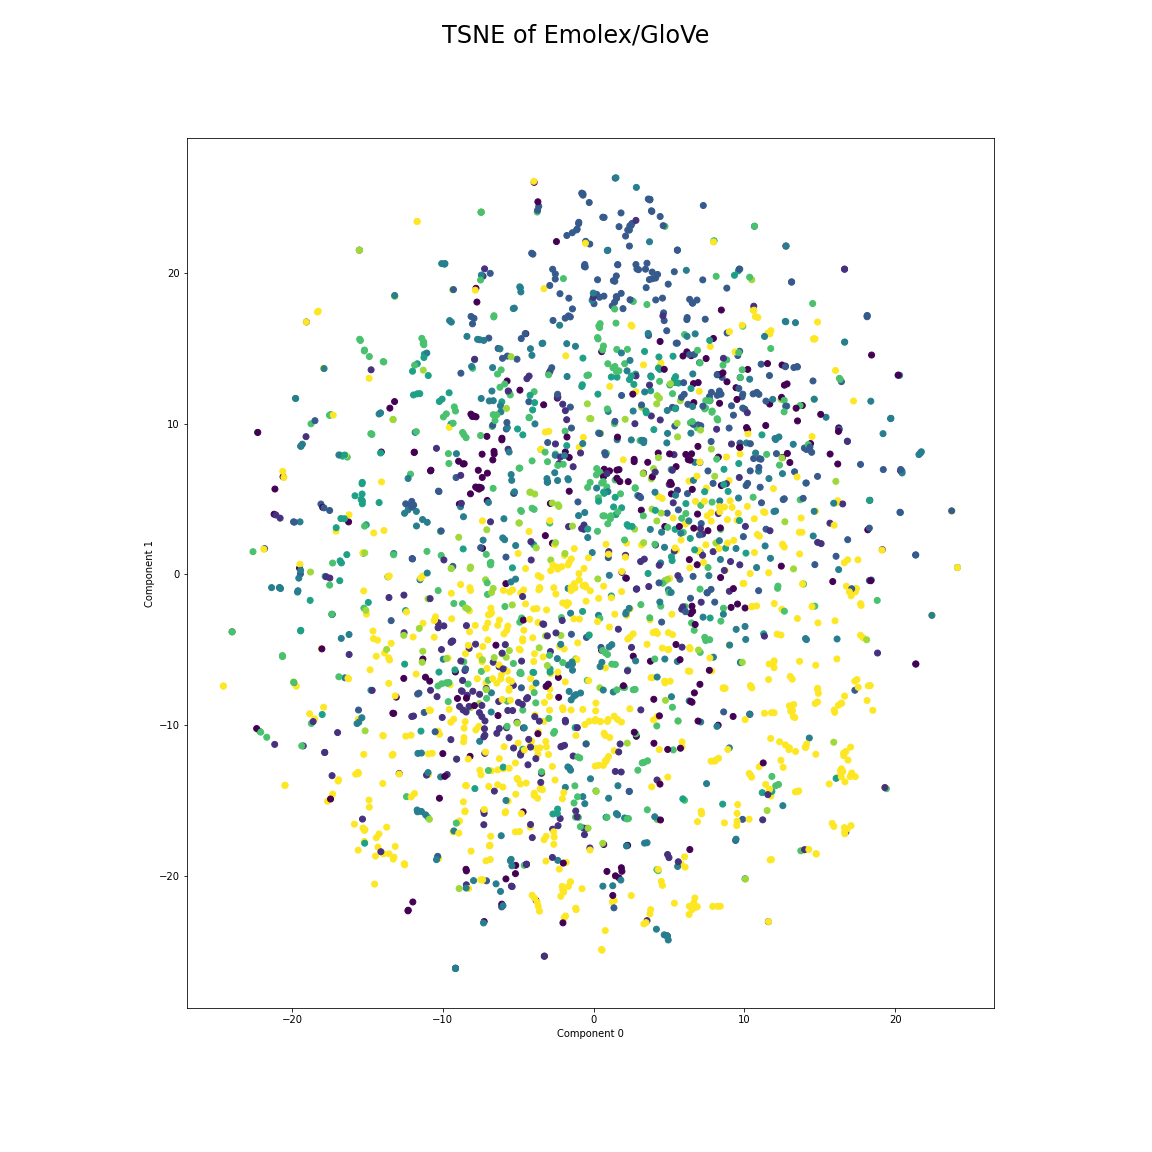
\includegraphics[width=1\textwidth]{plots/emolex/tsne_scat_emolex_glove}
  \centering
  \caption{EmoLex Scatter plot of TSNE}
\end{figure}\label{fig:tsne_scat_emolex_glove}

In this plot we can observe that two major distribution centers are created: one on the top of the plot and one on the bottom. The two groups are represented by two emotions: trust and disgust. These two are indeed polar opposites on the Plutchik model.

Within the these two groups, we can also observe sub-clusters. A further analysis of the plot has been done with the help of a bokeh interactive plot, present in HTML format in the plots folder of the repository. Here we can read the words in the sub-clusters.

One of the sub-clusters with the trust label is the one formed by the words: aposite, apostolic, chapland, vicar, episcopal, parish, deacon, ordained, priest, congregation. The sub-cluster also contains the word reverend, labeled with the emotion joy, and is very close to the sub-cluster with the words convent, nun, monk, abbot, and cannons, labeled with trust, and mystic, labeled with surprise.

With this example we can comment on what we expect to see in further experiments. Sub-clusters are formed by words that have semantic relationship, as it is expected from a functional language model, and the emotions labeled on to that word are an expression of the context of the person labeling the word, more than the intrinsic emotion of the word. This is conferment with the theory of constructed emotions.

These sub-clusters form an important part of the analysis, and have therefore been given a name: 'semantic islands'. A semantic island is a cluster of data points that have a semantic relationship.

As it is expected from a non-organic dataset, the structure to be found seems artificial. The distribution of the labels and words is uniform, and no conclusion must be drawn form it to apply to general language. Nonetheless, the visualization of the EmoLex as a dataset lets us develop the beginning of an intuition, and a technique as of how to approach this problem. In the following section, the same methodology will be followed to analyze the selected datasets and models.



\section{Results}\label{sec:Results}

The following results are separated into three: The correlation analysis, the PCA, or linear transformation, and the TSNE, or non-linear transformation.

%===============================================================================
\subsection{Correlation Analysis}\label{sub:Correlation Analysis}
A linear correlation is now compared between the four aforementioned language models. The results that best abstract the specifics of this dataset are those of the FastText model, since it has been trained specifically for this dataset. This is our baseline, and thus will be presented first:


\subsubsection{FastText}
With the FastText model, the maximum correlation was shown in the supervised approach, with 33.45\% correlation between the happiness emotion, and it's third dimension. The visualization of said model is shown in Figure~\ref{fig:cor_CrowdFlower_FastText}.

\begin{figure}[H]
  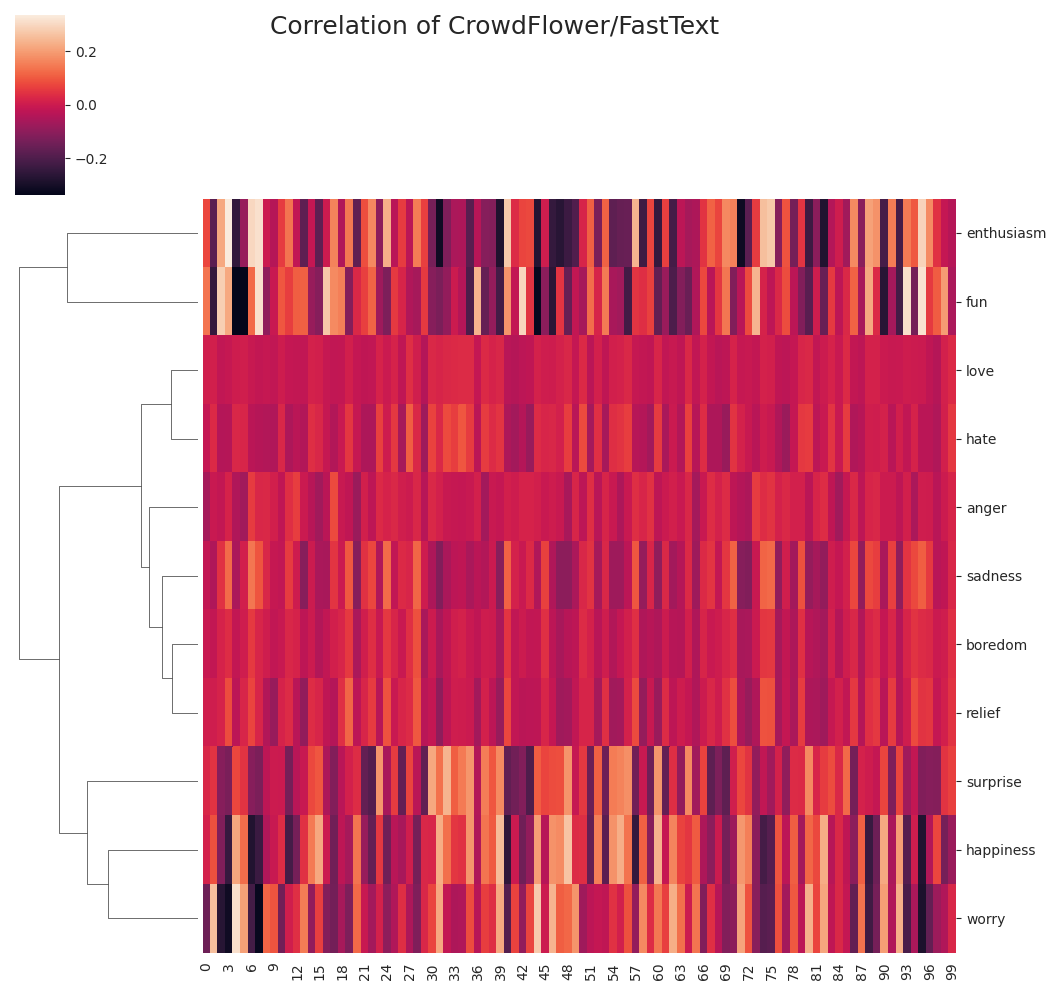
\includegraphics[width=1\textwidth]{plots/cor/cor_CrowdFlower_FastText}
  \centering
  \caption{Correlation plot for FastText}
\end{figure}\label{fig:cor_CrowdFlower_FastText}

A hierarchical structure of the concepts can also be observed, with two main groups: fun and enthusiasm in one, with a high activation of all dimensions (be it positive or negative), and the rest on a second group. The latter can be subdivided into two. The first group contains emotions of surprise, happiness, and worry, while the second one contains the rest of the emotions with very little activation.

An interesting observation is that love and hate have been clustered together, even if the activation of the vector space is very reduced.

\subsubsection{Word2Vec}
Word2Vec is the first pre-trained model to be reviewed. This model has been observed to contain an abstraction of valence, and it is thus expected to show it. Hollis et al. report that 208 dimensions out of the 300 dimensions of the model correlate with the concept of valence. They unfortunately do not mention how much the dimensions correlate~\cite{hollis2016principals}. In this case, the model's maximum correlation was between the happiness concept, and it's 43th dimension, with 11.94\%. This is means that most of the dimensions did not correlate significantly with the concepts we are exploring, since the random threshold is 9.09\%, and the maximum correlation found barely surpasses that, with most of them under the threshold.

\begin{figure}[H]
  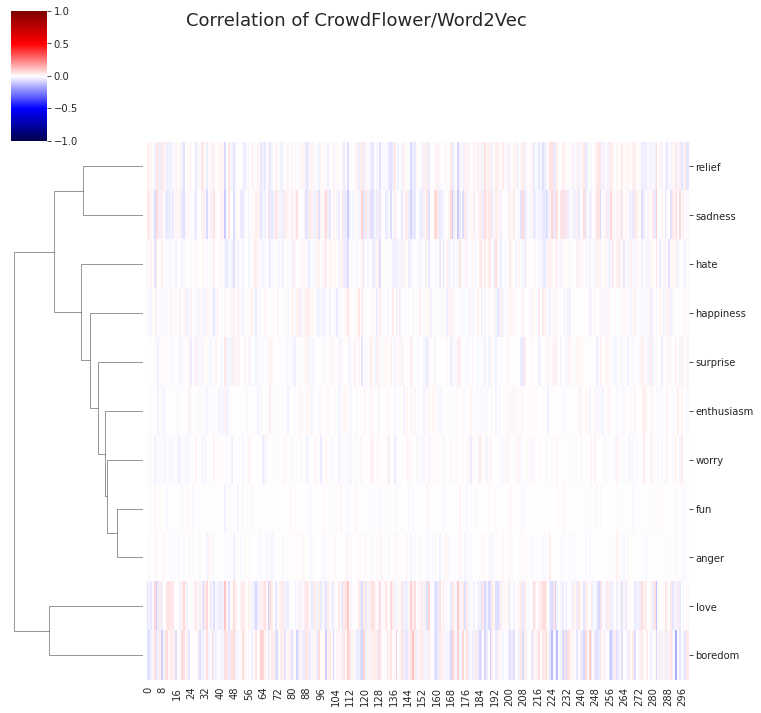
\includegraphics[width=1\textwidth]{plots/cor/cor_CrowdFlower_Word2Vec}
  \centering
  \caption{Correlation plot for Word2Vec}
\end{figure}\label{fig:cor_CrowdFlower_Word2Vec}

Figure~\ref{fig:cor_CrowdFlower_Word2Vec} shows the mentioned correlations. At first sight, it might seem that the clustering is similar to the one shown with FastText, with two main groups, one of which is again separated into two, but the emotions clustered are not the same. Clustered together are love and boredom, relief and sadness, and fun and anger. These are neither opposites, nor subsets of a valence side.

\subsubsection{GloVe}
The GloVe model presents a higher complexity than the Word2Vec. Thus, better results are expected. Here, the best correlation was 11.97 \%, between the worry concept, and the 164 dimension.This is again, barely above the random threshold.
\begin{figure}[H]
  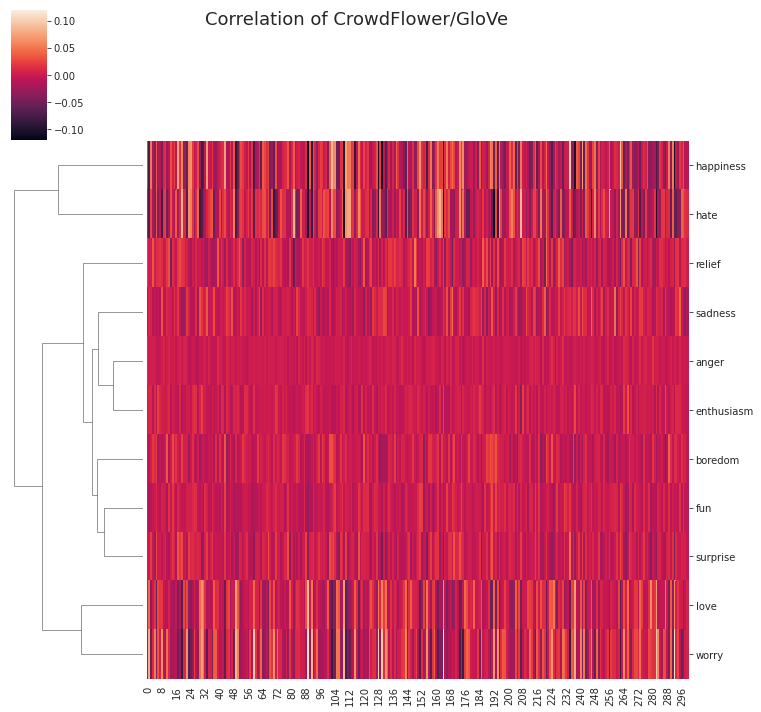
\includegraphics[width=1\textwidth]{plots/cor/cor_CrowdFlower_GloVe}
  \centering
  \caption{Correlation plot for GloVe}
\end{figure}\label{fig:cor_CrowdFlower_GloVe}
The clustering in Figure~\ref{fig:cor_CrowdFlower_GloVe} presents a similar structure, with different concepts as the last two models. Hate and happiness form a group, while the rest separate into two subgroups: one with love and worry, and the rest of the concepts, with almost no correlation, in a single big cluster.

\subsubsection{BERT}
BERT is the most powerful language model used within this project. Still, it presented a maximum correlation of only 13.87\% between the love concept, and dimension 305. Although slightly better than the previous results, it is still within the threshold of random sampling.
\begin{figure}[H]
  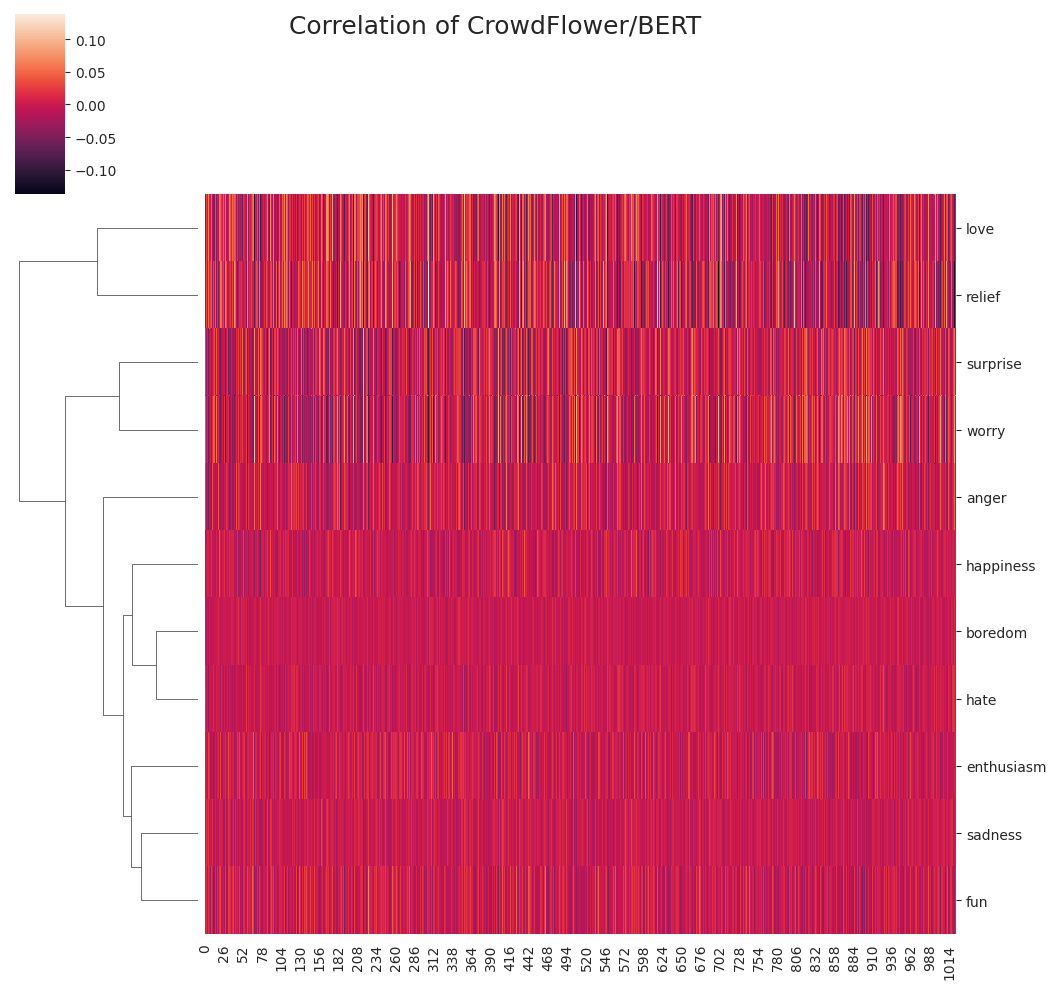
\includegraphics[width=1\textwidth]{plots/cor/cor_CrowdFlower_BERT}
  \centering
  \caption{Correlation plot for BERT}
\end{figure}\label{fig:cor_CrowdFlower_BERT}
On Figure~\ref{fig:cor_CrowdFlower_BERT}, we can observe that the concepts that most activate the latent dimensions in this model are love, relief, surprise, and worry. Love and Relief cluster into one group, Surprise and Worry in another. Not much structure can be observed, but sadness and fun did cluster into the less activated cluster.

\subsubsection{Analysis Discussion}
As we can see with these analysis, the linear interpretation of the dimensions of an embedded dataset, through a pre-trained language model does not provide consistent information about the representation of those concepts by the language model.


%===============================================================================
\subsection{Linear Transformation Analysis}\label{sub:Linear Transformation Analysis}
A linear transformation of the vector space generated by the language model can concentrate the information of said model on very little dimensions. This allows for a different analysis of the embedding of the concepts. For this analysis, we have selected the 11 top components of the PCA transformation. This allows us to see the numeric values in the visualization.

\subsubsection{FastText}
The baseline FastText analysis shows that the mostly correlated model was the supervised model, shown in Figure~\ref{fig:pca_cor_CrowdFlower_FastText}. This showed a maximum correlation of 36.85\% with the concept of hate. This is a slight improvement over the non-transformed analysis.
\begin{figure}[H]
  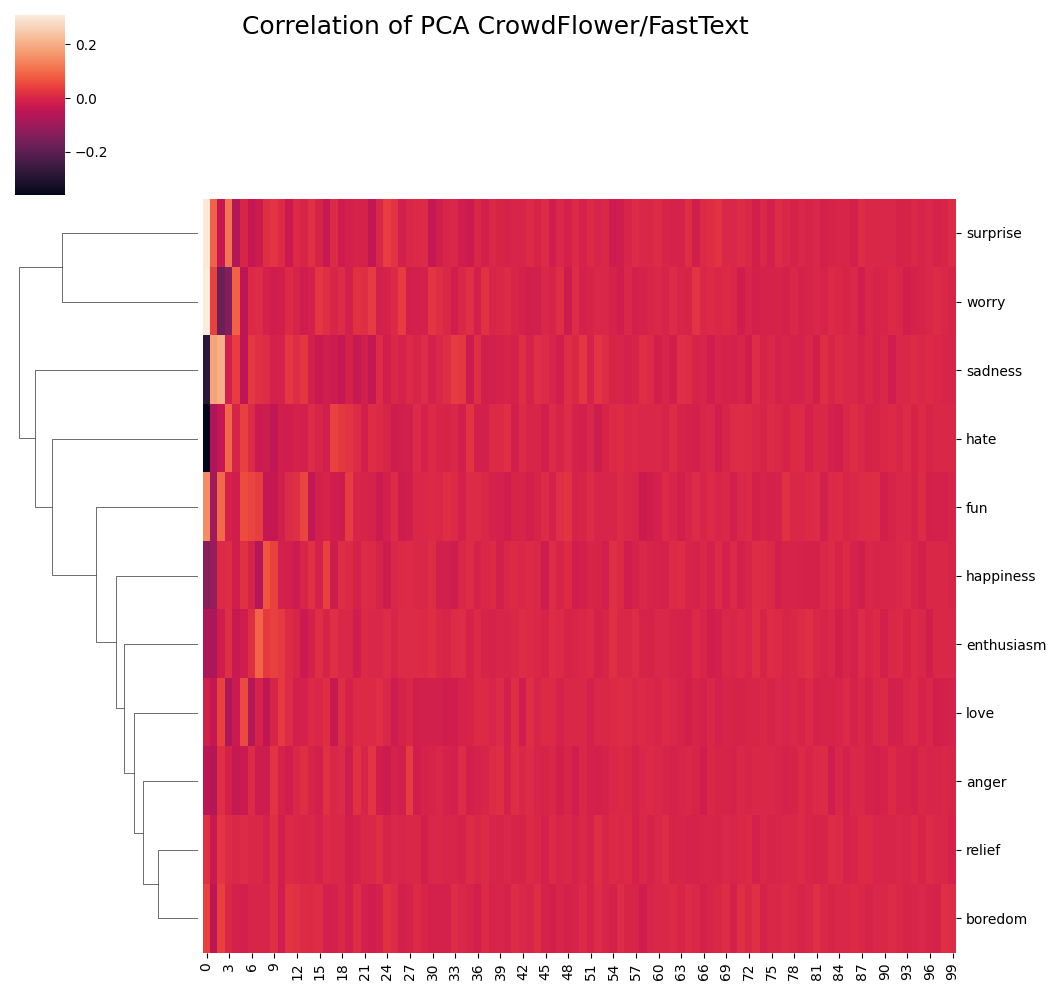
\includegraphics[width=1\textwidth]{plots/pca/pca_cor_CrowdFlower_FastText}
  \centering
  \caption{PCA Correlation plot for FastText}
\end{figure}\label{fig:pca_cor_CrowdFlower_FastText}
Figure~\ref{fig:pca_cor_CrowdFlower_FastText} shows that the first component of the transformation has a high positive correlation with the concepts of Surprise and Worry, while keeping a high negative correlation with Sadness and Hate. One grouping between Surprise and Worry is present, with the rest of the concepts in a second cluster.

\subsubsection{Word2Vec}
The transformation of the Wort2Vec representation presents the worst representation of concepts seen. The maximum correlation present is between the Love concept, and the second component.
\begin{figure}[H]
  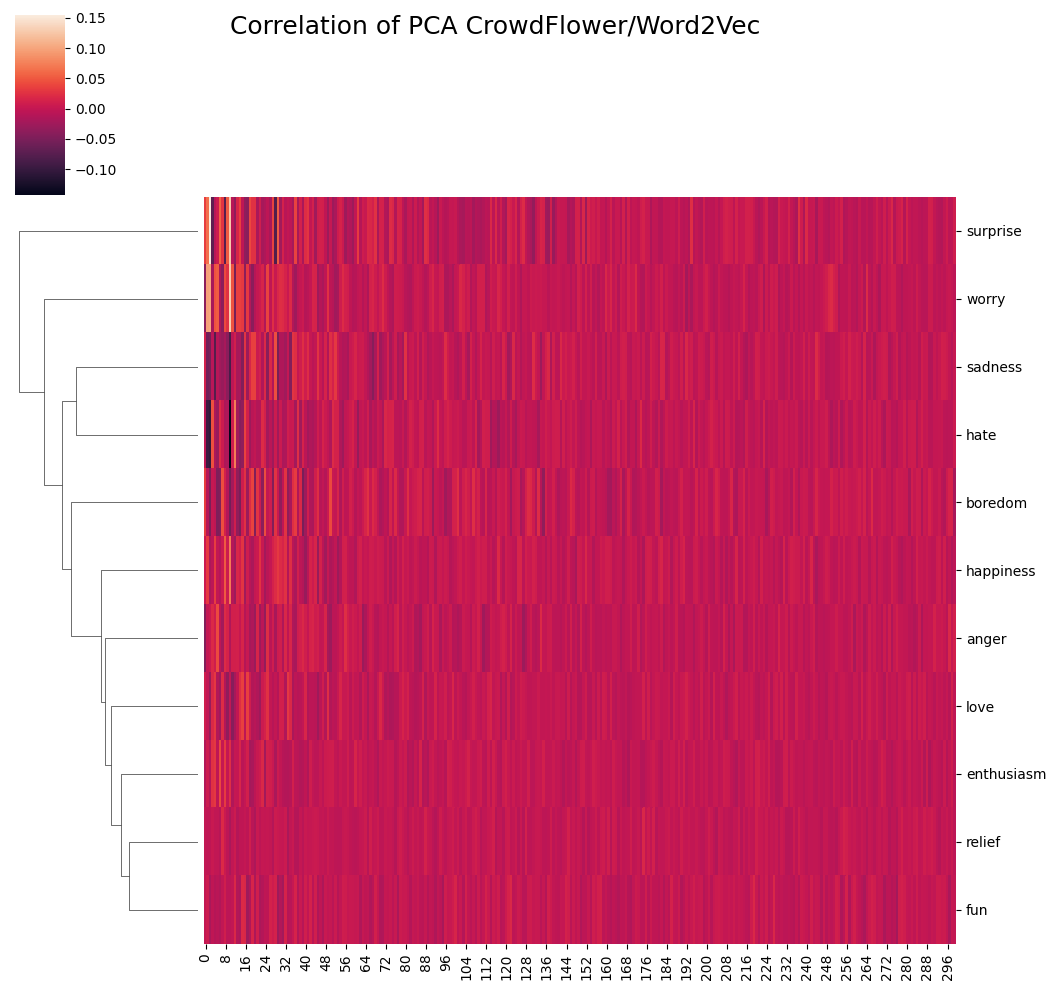
\includegraphics[width=1\textwidth]{plots/pca/pca_cor_CrowdFlower_Word2Vec}
  \centering
  \caption{PCA Correlation plot for Word2Vec}
\end{figure}\label{fig:pca_cor_CrowdFlower_Word2Vec}
Figure~\ref{fig:pca_cor_CrowdFlower_Word2Vec} shows the results of this analysis. Here, with a very low correlation, sadness and happiness have been clustered together, while relief and fun create the second most distinct group. The dichotomy of sadness and happiness is as expected from the baseline papers, but the correlation is much lower than if only valence is taken into account.
Another relevant grouping to mention is that of Anger and Worry. Although the direct correlations between the given concepts and the components of the transformed vector space are not statistically relevant, the clustering that can be done by analyzing these corresponds with that of parts of the Plutchik model, and accounts for dichotomy of emotions in a valence model of affect.

\subsubsection{GloVe}
The GloVe model shows a very low correlation, even worst that the Word2Vec model, which seems contradictory. The maximum correlation is 9.58\% lower than the threshold of random choice.
\begin{figure}[H]
  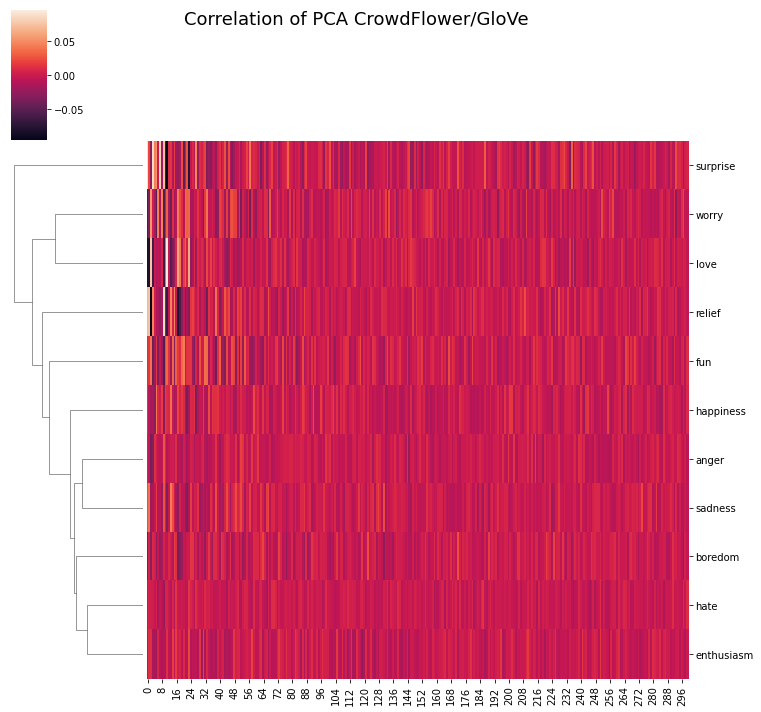
\includegraphics[width=1\textwidth]{plots/pca/pca_cor_CrowdFlower_GloVe}
  \centering
  \caption{PCA Correlation plot for GloVe}
\end{figure}\label{fig:pca_cor_CrowdFlower_GloVe}
Figure~\ref{fig:pca_cor_CrowdFlower_GloVe} shows how the low correlation of concepts and components of the PCA-transformed vector space yields no results that relate to emotion models. Even so, a three-group clustering is seen. This might indicate that this clustering is more related to the dataset, than to the language model.

\subsubsection{BERT}
The BERT model shows a maximum correlation of 10.28\% with between the component number 5 and the concept of Love. The correlations are not as high as expected, for the most powerful model in this project.
\begin{figure}[H]
  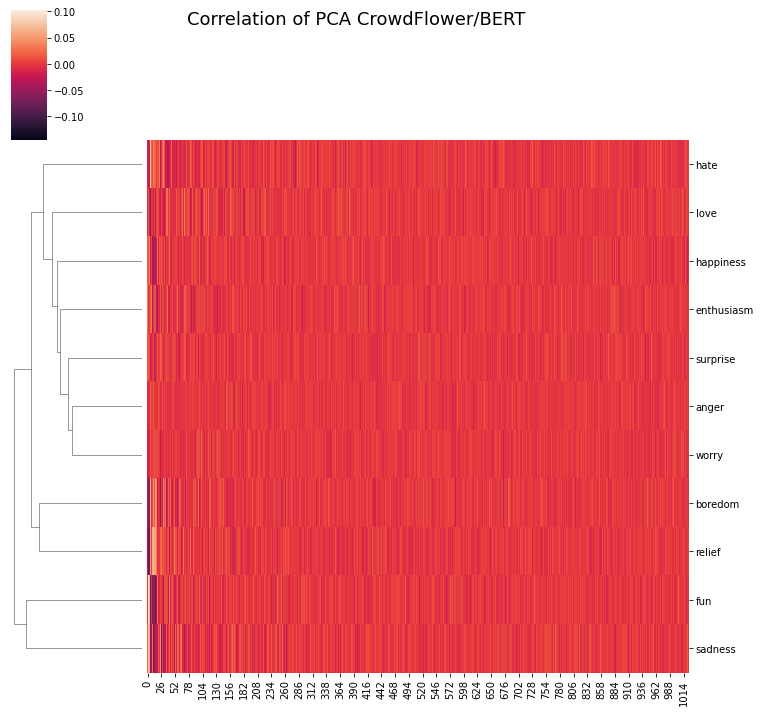
\includegraphics[width=1\textwidth]{plots/pca/pca_cor_CrowdFlower_BERT}
  \centering
  \caption{PCA Correlation plot for BERT}
\end{figure}\label{fig:pca_cor_CrowdFlower_BERT}
Figure~\ref{fig:pca_cor_CrowdFlower_BERT} shows how the results don't seem to be as densely populated by high correlations. This could be due to the high dimensionality of the model. With this PCA transformation 1024 dimensions are being reduced down to 10, which in comparison with the other models, is a much bigger reduction. No clustering seems relevant, when compared with emotion models.

\subsubsection{Analysis Discussion}
As mentioned before, a dimensionality reduction implies that some information will be lost by the model. If the information captured was already low, and the number of dimensions is significantly reduced, the results can end up being worst than random guess.

%===============================================================================
\subsection{Non-linear Transformation Analysis}\label{sub:Non-linear Transformation Analysis}
The TSNE non-linear dimensionality reduction allows for two-dimensional scatter plots that maximize the distance between groups in a dataset. A point in every scatter plot represents a sentence in the dataset. The color is the emotion label of that sentence.
\subsubsection{FastText}
As with the last two studies, the FastText approach is a supervised language model trained on this specific dataset. For this reason, it's also expected to have the TSNE scatter plot with the most clearly separate groups.
\begin{figure}[H]
  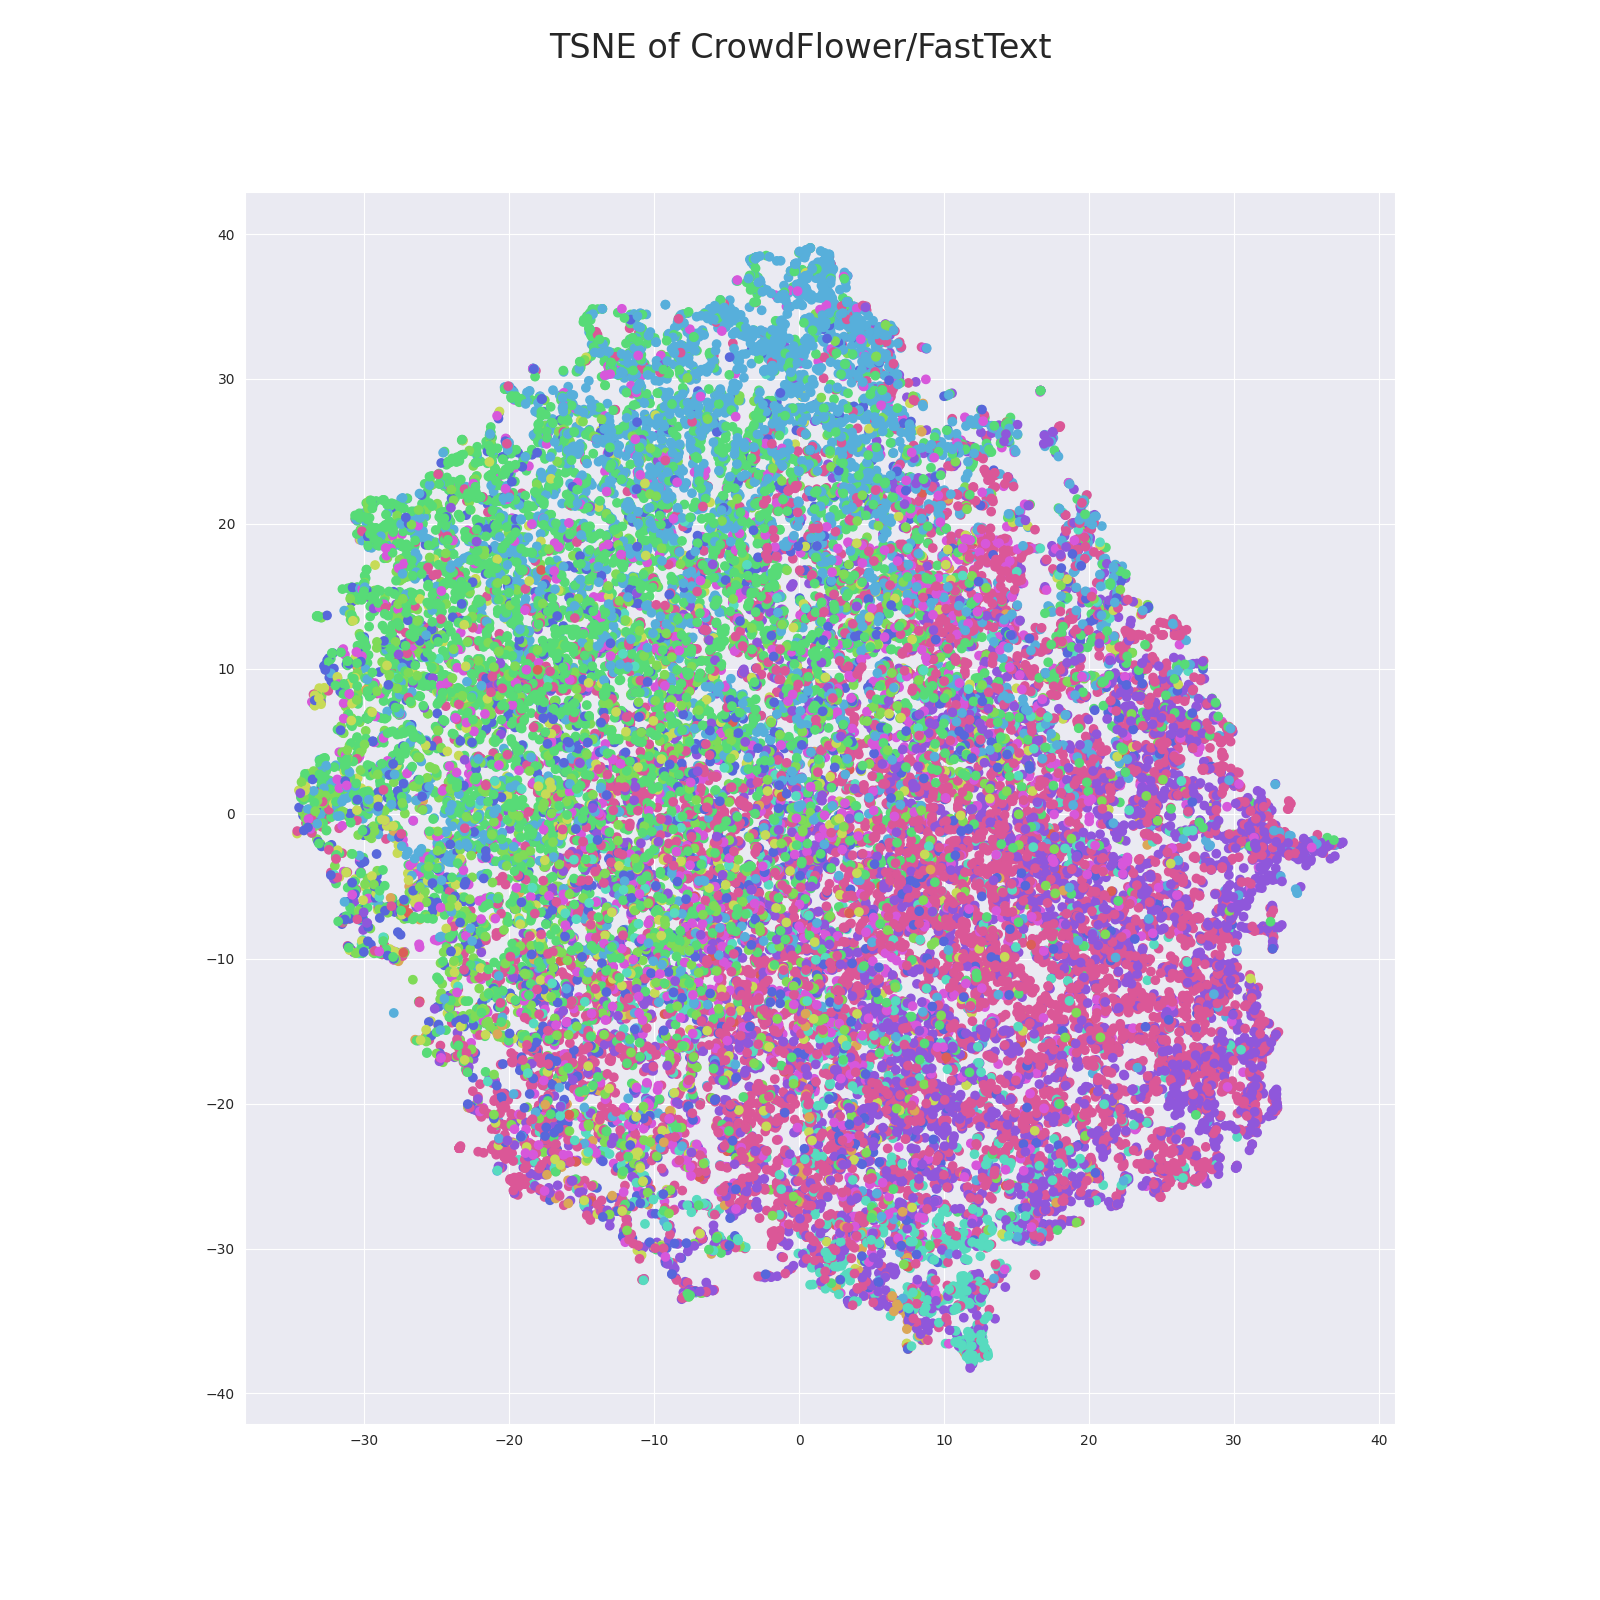
\includegraphics[width=1\textwidth]{plots/tsne/scat_CrowdFlower_FastText}
  \centering
  \caption{Scatter plot for TSNE of FastText}
\end{figure}\label{fig:scat_CrowdFlower_FastText}
It can be observed that Figure~\ref{fig:scat_CrowdFlower_FastText} shows clear gradients between groups. These are not linearly separable, but do comply with the emotion's valence value. Positive valenced emotions like Love, Fun and Happiness are present in the top part of the visualization (the positive side of component 1), while the negative emotions like Anger, Hate, and Sadness are presented in the lower part of the visualization. There is no clear separation of groups around the origin.
\subsubsection{Word2Vec}
As expected, the Word2Vec scattering does not present such clear groups as the ones shown by the FastText model. There is a main group of data points that fall around the origin, and a very slight gradient with positive valence at the bottom of component1, and negative valence at the top.
\begin{figure}[H]
  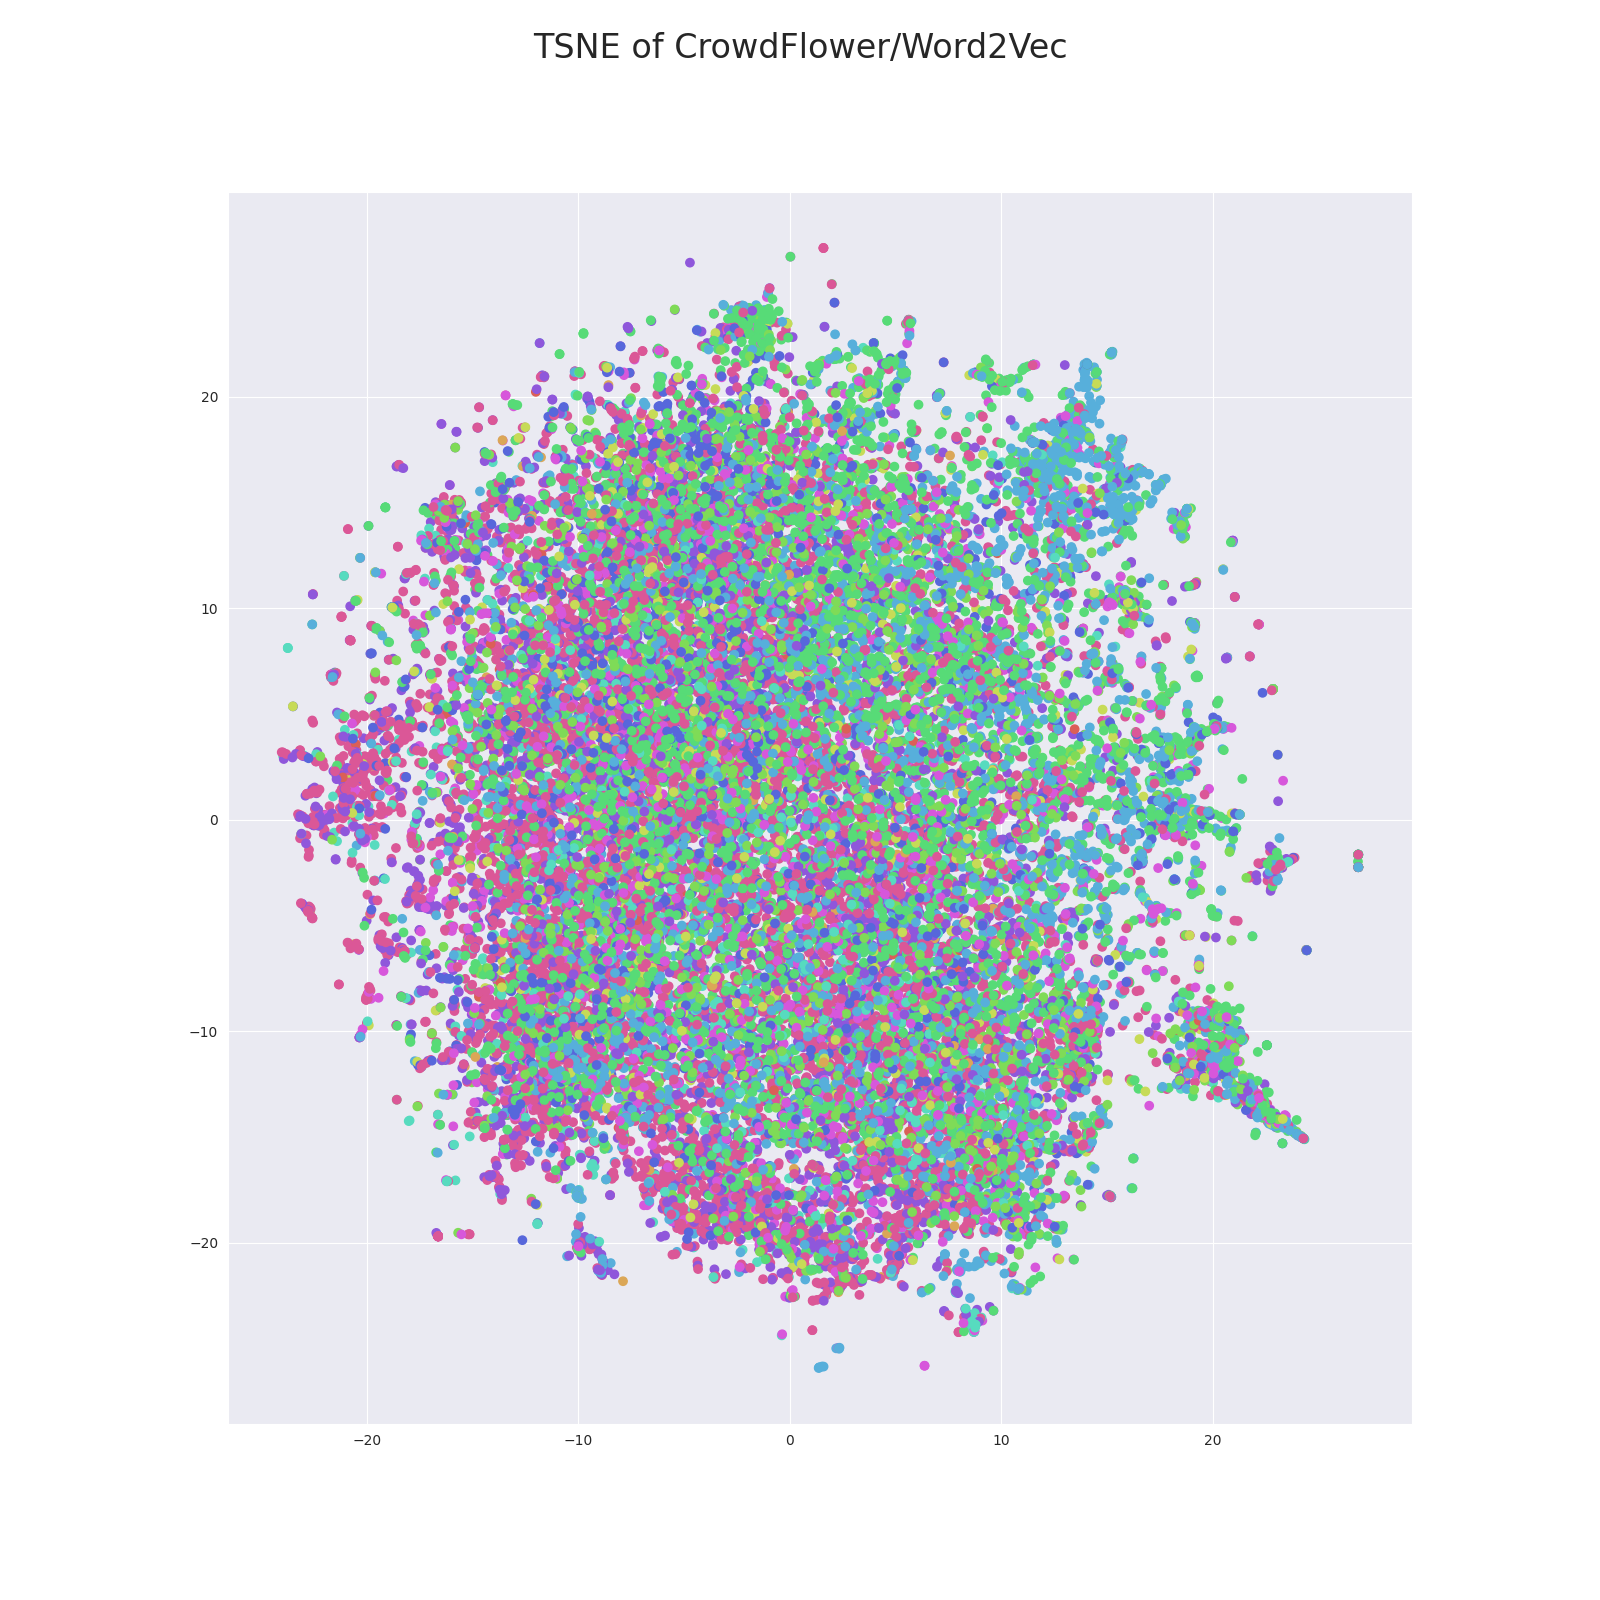
\includegraphics[width=1\textwidth]{plots/tsne/scat_CrowdFlower_Word2Vec}
  \centering
  \caption{Scatter plot for TSNE of Word2Vec}
\end{figure}\label{fig:scat_CrowdFlower_Word2Vec}
Figure~\ref{fig:scat_CrowdFlower_Word2Vec} shows a phenomenon present in pre-trained models. Some data points are separated from the main cluster, but are maintained relatively close to each other. These are sentences that are similar in meaning, sometimes even identical sentences, but contain a distinct emotional meaning.
\subsubsection{GloVe}
For the GloVe model, the gradient of positive and negative valenced emotions is not as clear as with the Word2Vec model.
\begin{figure}[H]
  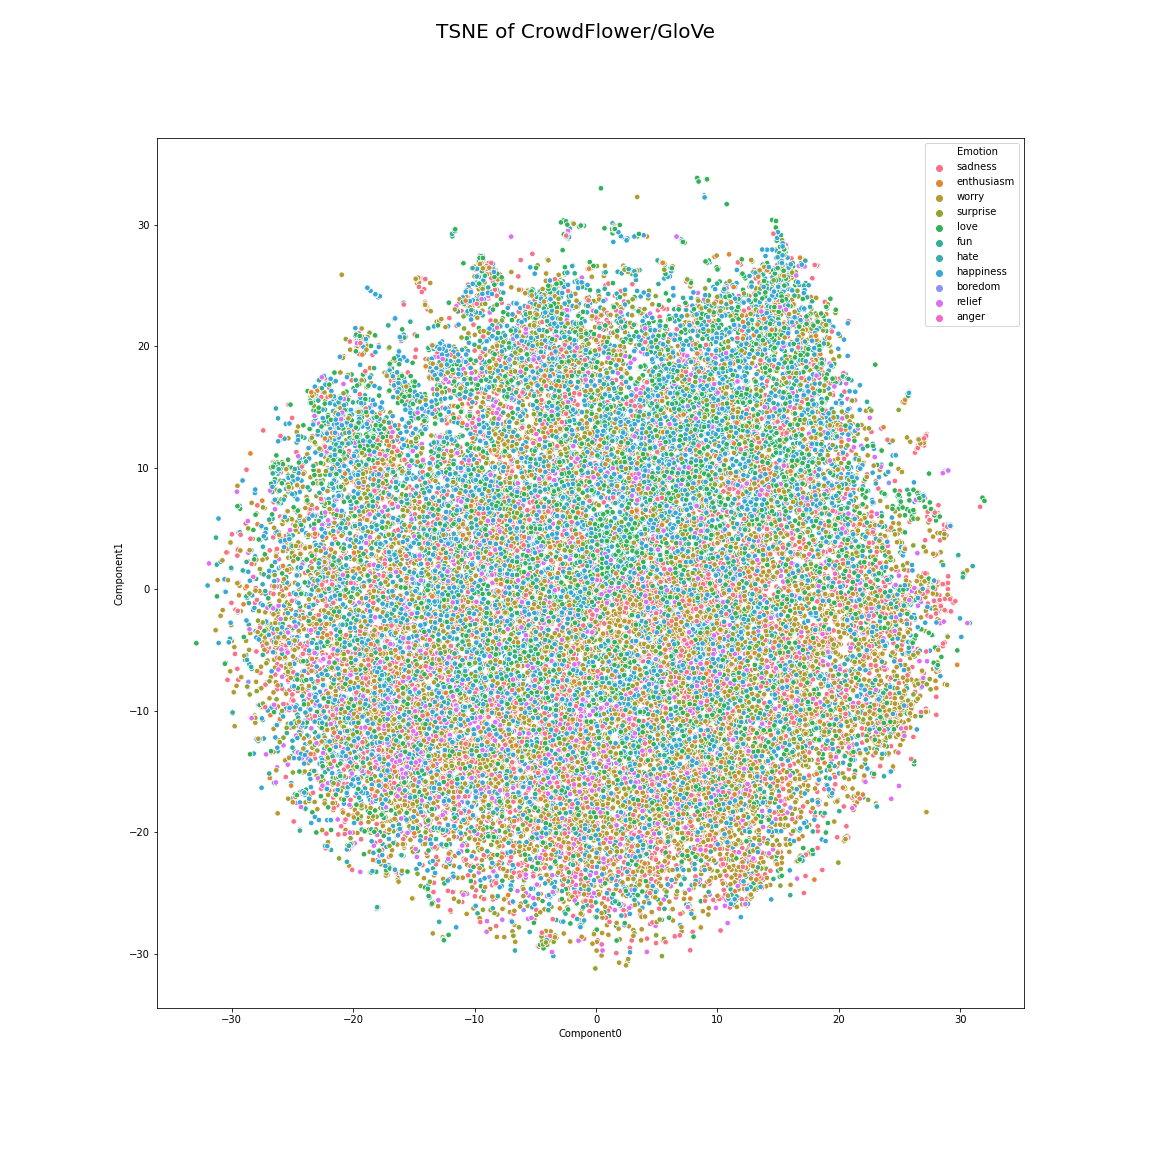
\includegraphics[width=1\textwidth]{plots/tsne/scat_CrowdFlower_GloVe}
  \centering
  \caption{Scatter plot for TSNE of GloVe}
\end{figure}\label{fig:scat_CrowdFlower_GloVe}
On Figure~\ref{fig:scat_CrowdFlower_GloVe} the dataset is represented mostly as a Gaussian distribution of scattered data points. If there are relevant features of this representation, they are on the top of the visualization, where most of the positively valenced emotions are. There, the semantic clusters, seem to be more common than anywhere else in the plot.

\subsubsection{BERT}
With this analysis, BERT comes out as the model that creates representations that are linearly separable, even after using average representation of sentences.
\begin{figure}[H]
  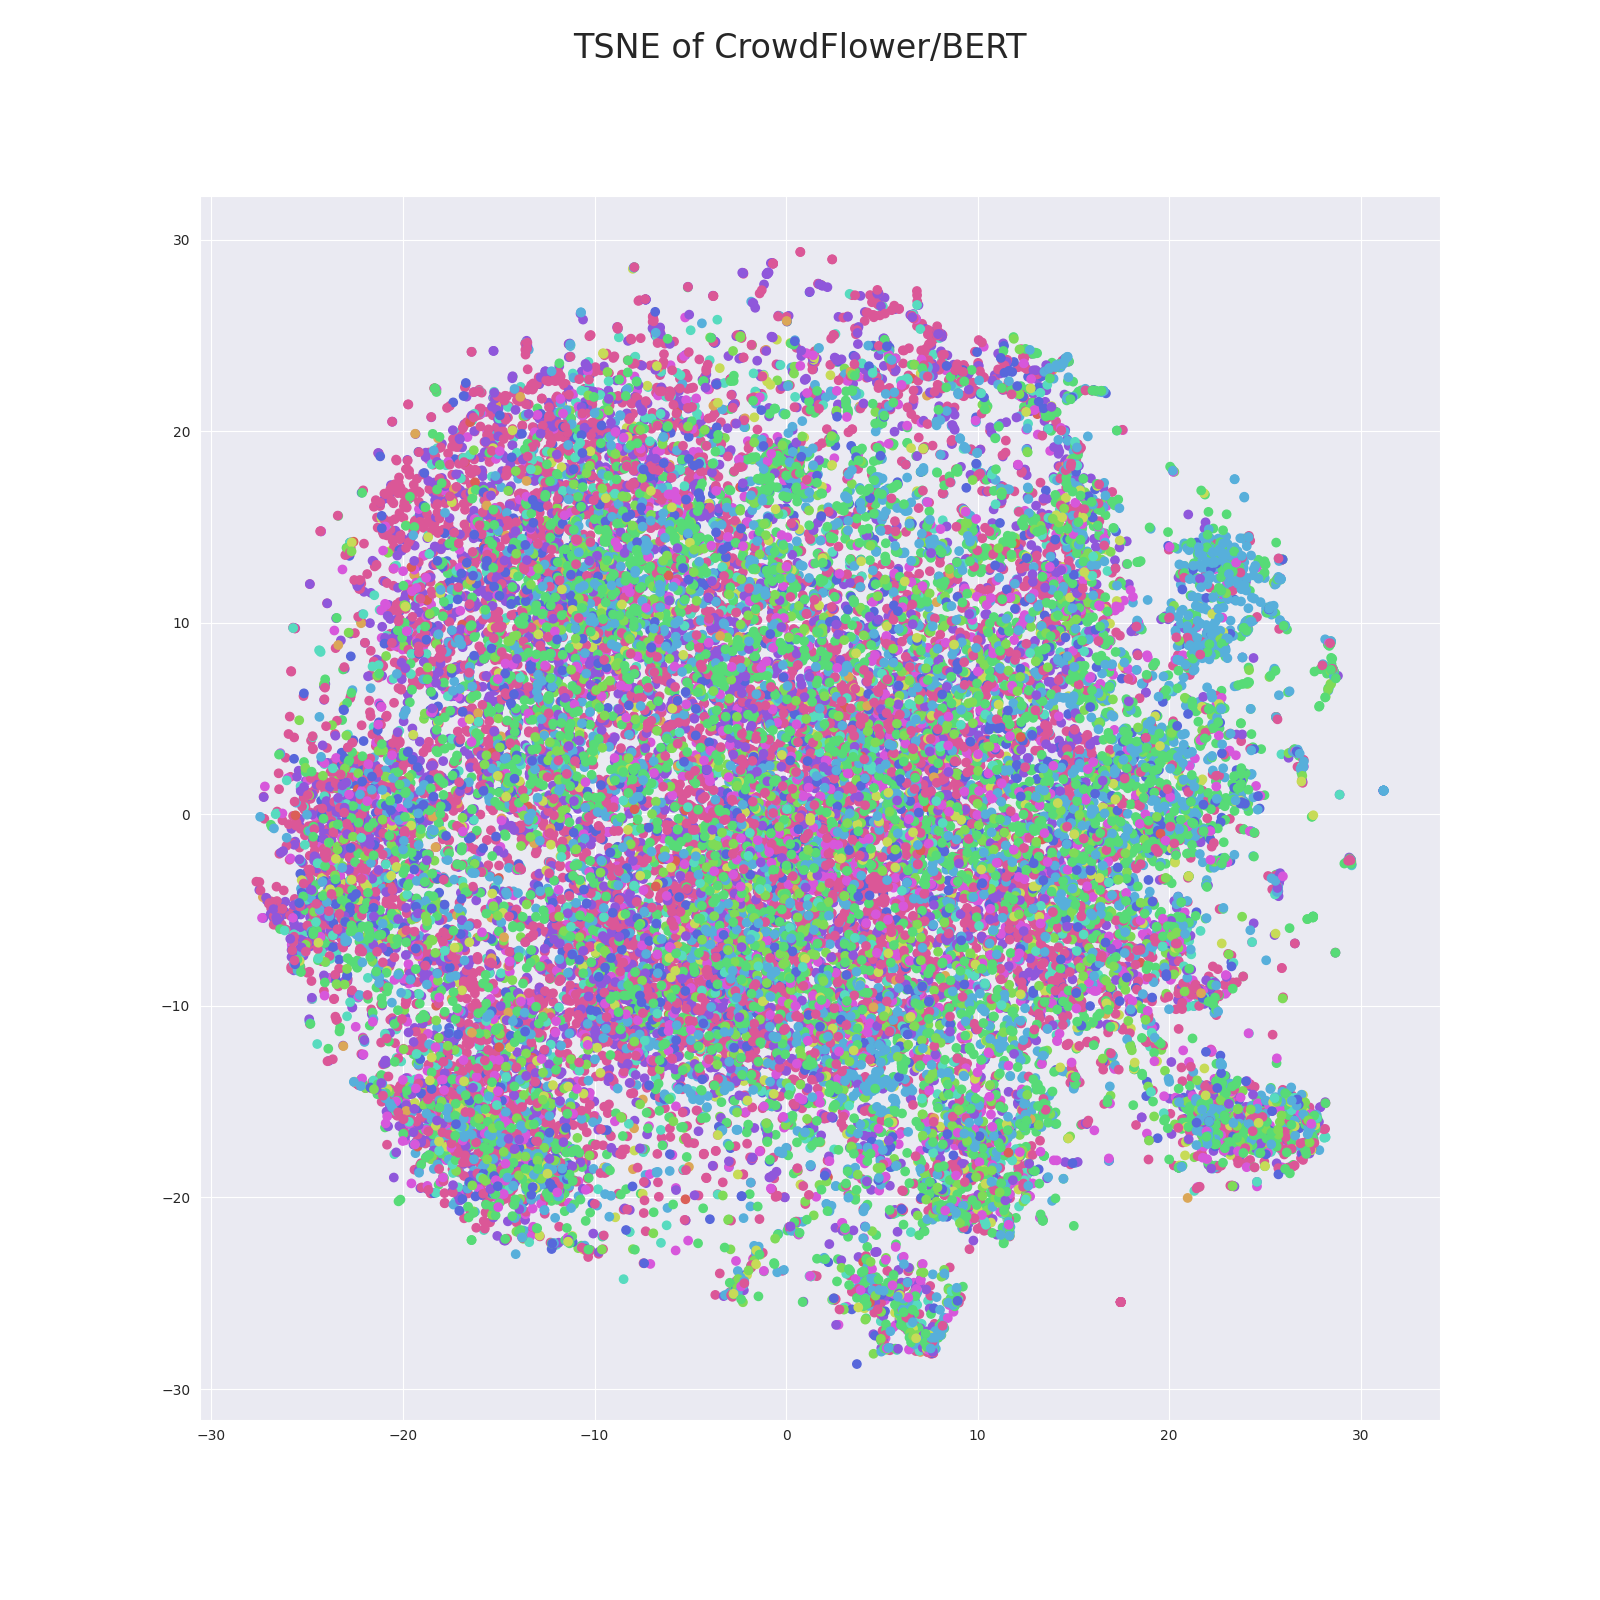
\includegraphics[width=1\textwidth]{plots/tsne/scat_CrowdFlower_BERT}
  \centering
  \caption{Scatter plot for TSNE of BERT}
\end{figure}\label{fig:scat_CrowdFlower_BERT}
In Figure~\ref{fig:scat_CrowdFlower_BERT} several clusters can be observed, with a very characteristic one composed of mostly Love, Fun, and Happiness labels around (-17, -12). This cluster can be considered as a positive valence cluster. Although there are several groupings of sentences, there seems to be no clear gradient of valence in the model, but valence might be a variable to be measured inside clusters of data points.

\subsubsection{Analysis Discussion}
All models presented in this project are created through non-linear methods. The pre-trained models are also optimized to be used with neural networks. For this reason, a non linear approach is expected to yield the best result for a classifier.

%===============================================================================
\subsection{Result Analysis}\label{sub:Result Analysis}
The models presented here seem to have very little representation of emotions, but a strong relationship with valence. Although this could indicate that the models for human language do not conceptualize emotions, some cases have been found, that might indicate that it is in fact, the dataset that makes it difficult to cluster the conceptualization of certain emotions.

\subsubsection{Class unbalance}
The class distribution of the CrowdFlower dataset is severely unbalanced. Table~\ref{tab:CrowdFlower_distribution} shows the classes, including neutral, which has been removed from this analysis.

\begin{table}
    \centering
    \begin{tabular}{|l|l|}
    \hline
      neutral     &  16894 \\
      worry       &  16840 \\
      happiness   &  10336 \\
      sadness     &  10284 \\
      love        &   7610 \\
      surprise    &   4360 \\
      fun         &   3532 \\
      relief      &   3042 \\
      hate        &   2640 \\
      empty       &   1606 \\
      enthusiasm  &   1510 \\
      boredom     &    358 \\
      anger       &    212 \\
    \end{tabular}
    \caption{Class distribution for CrowdFlower dataset.}\label{tab:CrowdFlower_distribution}
\end{table}

For this reason, the majority of the datapoints visualized in this project are Worry, Happiness, and Sadness.

\subsubsection{Semantic Clusters}
In the TSNE visualizations it's hard to pin down which data points represent what. For this reason, interactive visualizations have been made to explore freely the 2D space generated by this transformation. This visualizations can be found in the project repository. By examining these visualizations several observations can be made.

The first one is that the models abstract semantics pretty well, as expected. Creating semantic clusters, or 'Meaning Islands' for sentences that express the same idea, even if it's with different words. That's the case of the Star Wars island. This is a cluster in the Word2Vec TSNE transformation that clusters tweets sent on May 4th. (\textbf{Note}: the model did not have access to the date of the tweet, May the 4th is considered Star Wars day by the franchise's fan base) This cluster has a center around (26, -5). Tweets from this cluster include text like 'Happy Star Wars Day! May the 4th be with you', 'Happy Star Wars day!', or simply 'May the 4th be with you!'. Other tweets nearby include mentions of Bank's day, National days, or Fight Club's 10th anniversary.

Another interesting feature of this model is the 'ALL-CAPS' peninsula on Figure~\ref{fig:CapsPeninsula}, on the other side of the plot, at around (-25, 11). This feature's most compact cluster are tweets of people wishing a happy mother's day, but also features some tweets cursing (with and without mentioning of mothers in the cursing), wishing happy birth day, and one about Star Wars day. All these tweets have in common that at least some part of it is written in all capital letters.

\begin{figure}[H]
  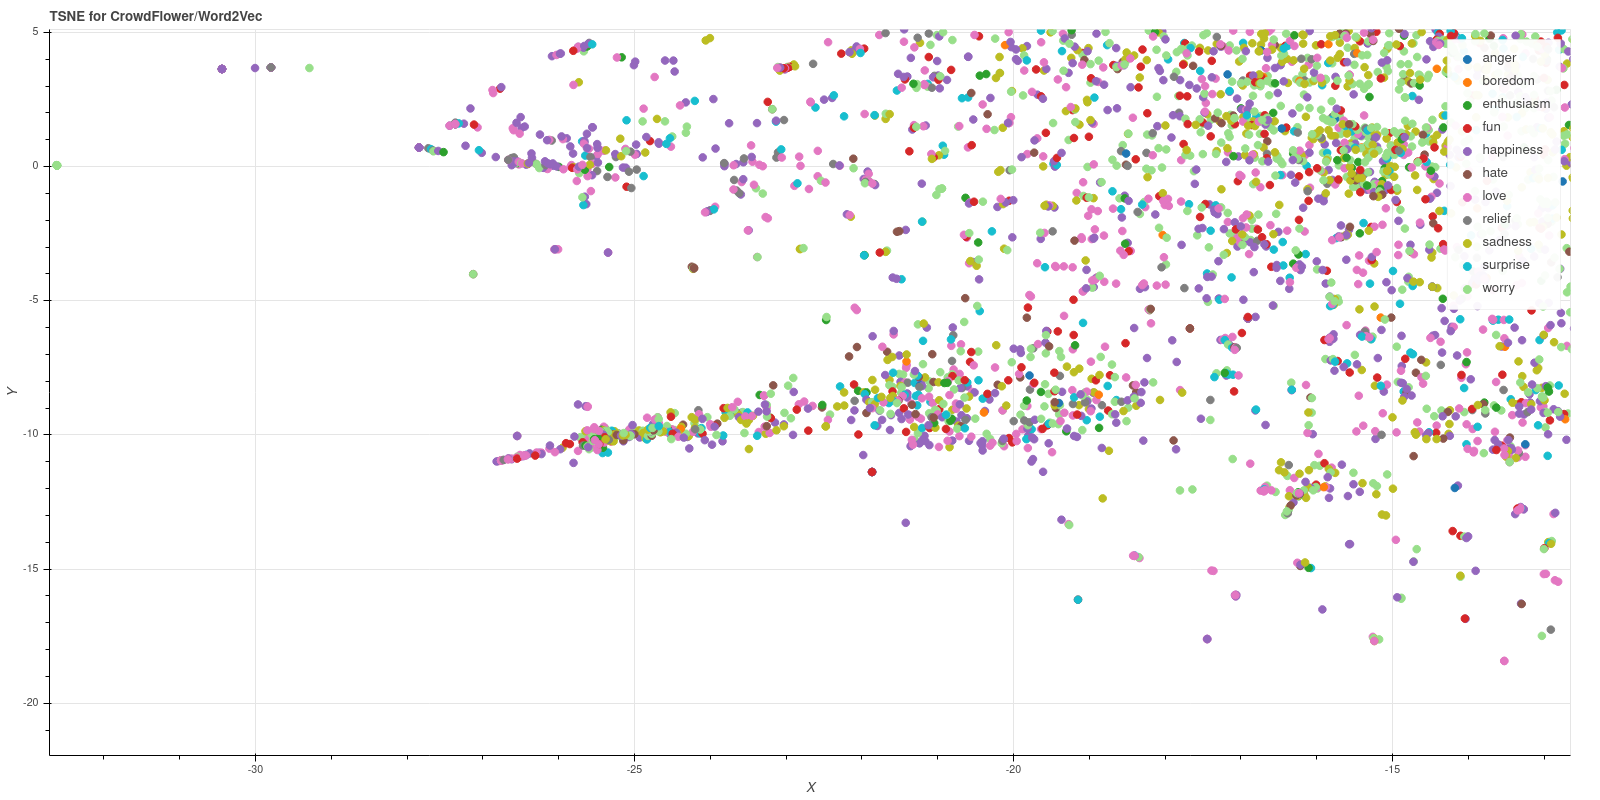
\includegraphics[width=1\textwidth]{plots/CapsPeninsula}
  \centering
  \caption{A zoom into the All-Caps peninsula for the TSNE transformation of the CrowdFlower DS under the Word2Vec LM}
\end{figure}\label{fig:CapsPeninsula}

Other interesting cluster is around (24, -10) in the Word2Vec projection, where most of the tags contain the word Happy, but are tagged with the emotion love.

In the GloVe projection, most tweets wishing for a happy mother's day seem to be disperse on the top region of the plot, but do not generally cluster.

A consequent observation of these clusters is that very similar tweets have different emotional labels. This does not necessarily mean that the labels are wrong. But it does speak about the meaning that that tweet had for the person that assigned the label. Emotions are according to theory, context dependant. Tweets for Mother's day are labeled with the emotions Love, Happiness, Fun, and even Worry.

A third observation comes from examining the dataset's text, where some of them are not in English. Some others are just links. In general there is an overload of people wishing a happy mother's day and a happy Star Wars day. Both of these dates happen in May.

\subsubsection{FastText Approach}
The FastText Language Model, trained with this dataset, seems to have taken the three most frequent labels, and separated them to two different extremes of the vector space. This is exactly what a supervised model should do, but by doing so it sacrifices the clustering between sentences that might be related, but written in a different manner.

 %!TEX root = ../thesis.tex
\chapter{Conclusion}\label{chap:Conclusion}

% Discussion
% Talk about the pedagogic value of this work

% Problems to be solved

% Future Work
% Talk about multi-label datasets, why they make sense, and why they should be looked into.
% How could they be looked into?

% New method for analysing the abstraction of concepts on pre-trained language models
Thanks to the work done in this project a new method for the creation of an emotional model can be created. A prospect model of emotions in text can be created by using explicit textual exrpessions of emotion. An example of an explicit expression of emotion is: \"I feel sad\" By removing the emotional word from this sentence, we can obtain an emotion-neutral emotion context. By parsing a corpus for these specific sentences, maping them on to a pre-trained-model vector space, and reproducing a separation method like PCA, the transformation that better captures the different emotional contexts can be obtained. This transformation can latter be used for non-explicit expressions of emotion.
This model of emotions can be context and languge specific, but the methodology is not restricted to any language, or even expressions of emotion. It is in general a method for analyzing conceptualizations of pre-trained language models.

% Ablative studies and their implications


% Talk about the horrors of accessing a dataset

% Talk about the crowdflower dataset and its weak points
% Talk about the EmotionX emotion tasks and its weak points


\bibliography{./chapters/06_bibliography}
\bibliographystyle{apalike}

\end{document}
